\documentclass[12pt,a4paper]{article}
\usepackage[utf8]{inputenc}
\usepackage[brazil]{babel}
\usepackage[unicode]{hyperref}

% Melhorias na justificação do texto e
% pequenos ajustes em fontes e alinhamentos. 
\usepackage[T1]{fontenc}
\usepackage{microtype}

% Para fórmulas matemáticas
\usepackage{amsmath}
\usepackage{amssymb}
\usepackage{mathtools}

% Para setas usadas em fórmulas dos grafos
\usepackage{MnSymbol}

% Permite o alinhamento horizontal de várias
% equações, assim elas não tomam muito espaço
% quando são muito pequenas.
\usepackage{tabularx}

% Símbolos diferentes para o texto, como setas →,
% símbolos de copyright e trademark, euro, etc.
% Não é muito útil, mas de vez em quando ajuda.
% Ao invés do comando do latex, dá pra usar o
% caractere em UTF-8 diretamente.
\usepackage{textcomp}

% For command patching
\usepackage{etoolbox}

% Permite criar formatações específicas, controla
% numerações e produz índices para teoremas e hipóteses.
\usepackage[hyperref]{ntheorem}

% Hack para possibilitar quebra de longas linhas de
% texto no cabeçalho do teorema >_<
\makeatletter
\patchcmd{\@xthm}{\ignorespaces}{\nobreak\ignorespaces}{}{}
\patchcmd{\@ythm}{\ignorespaces}{\nobreak\ignorespaces}{}{}

\newtheoremstyle{hypo}%
  {\item{\theorem@headerfont
          ##1\ ##2\theorem@separator}\hskip\labelsep\relax}%
  {\item{\theorem@headerfont
          \MakeUppercase{##1}\ ##2:\ ##3\theorem@separator}\hskip\labelsep\relax}
\makeatother

% Definição do estilo para "Hipótese"
\theoremstyle{hypo}
\theoremseparator{:}
\theoremheaderfont{\normalfont\scshape}
\theorembodyfont{\itshape}
\newtheorem{hypothesis}{Hipótese}

% Notações matemáticas usadas com frequência no texto.
% Isso possui três vantagens:
% 1 - Dá menos trabalho digitar as fórmulas
% 2 - Dá mais consistência à notação no trabalho
% 3 - Se mudar de ideia qto à notação, é só trocar aqui
%     e o trabalho todo fica certo.
% Notação matemática
\newcommand{\R}{\mathbb{R}}
\newcommand{\avg}[1]{\left\langle #1 \right\rangle} % ... média
\newcommand{\defn}{\coloneqq} % Usamos "=", ":=" ou "\equiv?"
\newcommand{\noloop}[1]{#1^\nlcirclearrowleft} % ... sem loops
% Redes direcionadas
\newcommand{\linkin}[1]{#1^\leftarrow} % ... entrada
\newcommand{\linkout}[1]{#1^\rightarrow} % ... saída
\newcommand{\linkboth}[1]{#1^\leftrightarrow} % ... direcionada
% Redes ponderadas e direcionadas
\newcommand{\win}{w^\leftarrow} % peso e direção de entrada
\newcommand{\wout}{w^\rightarrow} % peso e direção de saída
\newcommand{\weighted}[1]{#1^w} % ... com pesos
\newcommand{\weighteddir}[1]{#1^{w\rightarrow}} % ... com peso e direção
% Reciprocidade
\newcommand{\recin}[1]{#1^\leftlsquigarrow} % ... entrada não-recíproca
\newcommand{\recout}[1]{#1^\leadsto} % ... saída não-recíproca
\newcommand{\recboth}[1]{#1^\leftrightsquigarrow} % ... recíproca

% Para listagens de programação ou 
% textos onde a formatação importa
\usepackage{listings}
\lstset{
	inputencoding=utf8,
    extendedchars=true,
	framextopmargin=2pt,
    framexbottommargin=2pt,    
    literate={á}{{\'a}}1
             {ã}{{\~a}}1
             {é}{{\'e}}1
             {í}{{\'i}}1
             {ç}{{\c{c}}}1
             {Ç}{{\c{C}}}1,
}
\renewcommand{\lstlistingname}{Listagem}% Listing -> Listagem
\renewcommand{\lstlistlistingname}{Lista de \lstlistingname s}% List of Listings -> Lista de Listagens

% Permite colocar figuras lado a lado ou
% fazer posicionamentos arbitrários
\usepackage[lofdepth,lotdepth]{subfig}

% Permite o uso da opção "frame" em "includegraphics"
% para fazer uma borda na imagem
\usepackage[export]{adjustbox}

% Para inserir gráficos e imagens
\usepackage{graphicx}
% Diretório padrão para figuras
\graphicspath{ {images/} }

\usepackage{abnt-alf}
\usepackage[top=3cm,bottom=2cm,left=3cm,right=2cm]{geometry}
\usepackage{indentfirst}
\usepackage{csquotes}

% Prefine que parágrafos (\paragraph) sejam colocados
% no índice. Isse permite usá-los livremente para
% formatação, caso contrário temos um erro se eles não
% estiverem dentro de uma subsubsection.
\setcounter{tocdepth}{3}

% Adiciona o comando \source para citar fontes abaixo
% de figuras. Muito útil!
\usepackage{caption}
\newcommand{\source}[1]{\vspace{-10pt} \caption*{Fonte: {#1}} }

% Facilita o copy 'n paste no PDF
% Remove ligaturas na cópia
%\input{glyphtounicode}
%\pdfgentounicode=1

% Texto colorido e afins. Bom para TODO notes
\usepackage{xargs}
\usepackage[pdftex,dvipsnames,table,xcdraw]{xcolor}
\usepackage[normalem]{ulem}
\useunder{\uline}{\ul}{}

% Todo notes.
% Muito útil para deixar anotações enquanto se está
% construindo o texto, depois dá para remover e onde
% quebrar são comentário que devem ser removidos.
\usepackage[colorinlistoftodos,prependcaption,textsize=tiny]{todonotes}
\newcommandx{\question}[2][1=]{\todo[linecolor=red,backgroundcolor=red!25,bordercolor=red,#1]{#2}}

\newcommandx{\change}[2][1=]{\todo[linecolor=blue,backgroundcolor=blue!25,bordercolor=blue,#1]{#2}}

\newcommandx{\info}[2][1=]{\todo[linecolor=OliveGreen,backgroundcolor=OliveGreen!25,bordercolor=OliveGreen,#1]{#2}}

\newcommandx{\draft}[2][1=]{\todo[linecolor=Plum,backgroundcolor=Plum!25,bordercolor=Plum,#1]{#2}}

\newcommandx{\thiswillnotshow}[2][1=]{\todo[disable,#1]{#2}}
\reversemarginpar
% END Todo notes.

\begin{document}

% CAPA
\pagestyle{empty}
\begin{center}
\large  \textbf{UNIVERSIDADE PRESBITERIANA MACKENZIE}
\large  \textbf{PROGRAMA DE PÓS-GRADUAÇÃO EM}\\
\large  \textbf{ENGENHARIA ELÉTRICA E COMPUTAÇÃO}\\
\vskip 2.0cm
\textbf{\large Ronie Miguel Uliana}\\
\vskip 4.0cm
\setlength{\baselineskip}{1.5\baselineskip}
\textbf{\MakeUppercase{\large Um Estudo do Mapa de Carreiras da Empresa Vagas.com Usando Ciência de Redes}}\\
\vskip 4.5cm
\end{center}
\hfill{\vbox{\hsize=8.5cm\noindent\strut
Documento de Qualificação apresentado ao \break
Programa de Pós-Graduação em Engenharia \break
Elétrica e Computação da Universidade \break
Presbiteriana Mackenzie como parte dos \break
requisitos para a obtenção do título de \break
mestre em Engenharia Elétrica e Computação.}\\
\strut}
\vskip 3.0cm
\textbf{\normalsize Orientador: Prof. Dr. Leandro Nunes de Castro}\\
\vskip 2.0cm
\begin{center}
São Paulo\\
2017\\
\end{center}

% RESUMO
\newpage
\thispagestyle{plain}
\pagenumbering{roman}
\begin{center}
\large
\textbf{RESUMO}
\end{center}
\renewcommand{\baselinestretch}{0.6666666}
A ser definido
\\[0.5cm]
\begin{flushleft}
{\bf Palavras-chave:} {\it apresentação, separada por vírgulas, de três a seis unitermos significativos para o trabalho.}
\end{flushleft}

% SUMÁRIO
\newpage
\thispagestyle{empty}
\tableofcontents

% DESENVOLVIMENTO
\newpage
\pagestyle{plain}
\pagenumbering{arabic}
\renewcommand{\baselinestretch}{1.5}
\normalsize

\listoftodos[Notas]

%====================================
\section{INTRODUÇÃO}
%====================================

Ao longo da vida profissional é comum para o indivíduo passar por diversas movimentações na carreira. Um estudante de engenharia pode iniciar como Trainee em uma empresa e progredir para Engenheiro, Supervisor de Obras e Diretor de Engenharia. Na área de computação é possível ver um Programador se tornar Analista-Programador, Coordenador de Desenvolvimento, Gerente de Projetos, chegando a Diretor de Operações. Esses são casos em que a movimentação de carreira segue um padrão mais tradicional de progressão, mas também há situações extremas de transições de carreira na qual um Analista-Programador resolve se tornar um Chef de Cozinha. Em qualquer um dos casos, as movimentações de carreira são sempre uma etapa de grande relevância profissional e que, ao mesmo tempo, podem causar estresse, insegurança e alguns desconfortos pelos novos desafios que surgirão.

Este projeto de pesquisa usa uma base de dados de mercado com 10 milhões de currículos e 23 milhões de experiências profissionais da empresa Vagas Tecnologia com o objetivo de fazer um estudo analítico sobre a movimentação de profissionais entre ocupações durante o curso de suas carreiras. O problema é modelado com uma estrutura em grafos e é analisado com conceitos e técnicas de Ciência da Redes.

Existem diversos trabalhos sobre movimentação profissional, principalmente sobre os fatores que motivam a mudança, como os expostos por~\citeonline{Ng2007-zp}~\todo{Ronie: tem mais uma série de papers, ler e mencionar (na introdução, talvez?)}. Porém, nenhum trabalho pôde ser encontrado analisando redes profissionais sob a ótica da Ciência de Redes, ponto onde esse trabalho tem sua principal contribuição.

A movimentação de profissionais é um ponto de interesse para pessoas, empresas e governo. Pessoas desejam saber onde podem chegar, empresas se interessam pela contratação e evolução de seus colaboradores e o setor público traça planos para suprir mão de obra onde ela é insuficiente ou criar oportunidades de trabalho onde ela é abundante. A pesquisa presente traz uma maior compreensão sobre como essa movimentação ocorre.

%====================================
\subsection{Definições}

Para facilitar a compreensão do texto, abaixo são apresentadas definições para os termos encontrados no restante desse trabalho. Os conceitos são baseados nos trabalhos de \citeonline{Barabasi2016-rn}, \citeonline{Van_Steen2010-tf} e \citeonline{Goldbarg2012-uc}.

\begin{description}    
    \item[Nó] ou \textbf{Vértice} são termos usados para descrever entidades em um grafo. A literatura de Ciência de Redes normalmente opta por \enquote{nó} em detrimento a \enquote{vértice}, enquanto a literatura de Teoria de Grafos utiliza claramente o termo \enquote{vértice}. Nesse trabalho, os termos são usados como sinônimos.
    
    \item[Conexão] ou \textbf{Aresta} são termos usados para descrever as relações entre pares de nós. A literatura de Ciência de Redes utiliza \enquote{conexão}, enquanto a Teoria de Grafos utiliza \enquote{aresta}. Da mesma forma que o item anterior, esse trabalho usa ambos os termos como sinônimos.
    
    \item[Grau] o número de conexões de um nó. Em um grafo direcionado, o \textit{grau de entrada} representa o número de conexões que chegam ao nó, enquanto que o \textit{grau de saída} se refere ao número de conexões que partem do nó.
\end{description}

\subsection{Considerações sobre Carreira}

A definir\ldots

%====================================
\subsubsection{Atração entre ocupações}

\todo[inline]{procurar referências na área de RH, não encontrei em uma primeira tentativa (termos errados, talvez?)}

Para os propósitos desse trabalho, definimos o conceito de \enquote{atração} para o grau em que uma ocupação atrai mais profissionais do que outra.

Em termos quantitativos, isso significa que o fluxo de profissionais entre duas ocupações é mais intenso em uma direção que em outra. Isso não significa necessariamente que uma ocupação é mais desejável que outra em qualquer sentido social.

\todo[inline]{Deve ter algo sobre isso em redes de fluxo =/}

%====================================
\section{CIÊNCIA DE REDES}
%====================================

A Ciência de Redes (\textit{Network Science}) é uma área de estudo recente. Apesar do estudo matemático de grafos remontar ao século 18, com Leonhard Euler, o estudo de redes tem-se intensificado, culminando em um surto de interesse nos começo do século 21 com os trabalhos de Watts-Strogatz e Barabási-Albert [{REFS}].

Um marco para a consolidação da disciplina ocorreu em 2005 com o aval de órgãos governamentais quanto a sua utilidade como ciência. Nesse ano, o exército Norte-Americano solicitou ao \textit{United States National Research Council} um estudo sobre a aplicabilidade da emergente \enquote{Ciência de Redes}. O relatório destaca a relevância do campo em diversas áreas e levanta seus desafios. Nos anos seguintes foram fundados centros de estudos de Ciência de Redes nas universidades norte-americanas com investimentos dos laboratórios de pesquisa do exército [{REFS}].

O \citeonline{National_Research_Council2006-lv} define a Ciência de Redes como \enquote{o estudo da representação em rede de fenômenos físicos, biológicos e sociais levando a modelos preditivos desses fenômenos}~\footnote{Em tradução livre, \enquote{the study of network representations of physical, biological, and social phenomena leading to predictive models of these phenomena.}}.

Segundo \citeonline{Barabasi2016-rn}, como disciplina, a Ciência de Redes se diferencia de uma abordagem tradicional pelos seguintes pontos:

\begin{description}
	\item[\textit{Interdisciplinar}.] A Ciência de Redes é terreno comum para diversas disciplinas, como Biologia (com redes de proteínas), Sociologia (com redes sociais), Computação (com redes de comunicações e algoritmos), entre outras. Apesar de divergirem em essência e propósito, as redes que são seu objeto de estudo compartilham características e propriedades.
    
    \item[\textit{Empírica}.] A Ciência de Redes foca em dados reais e no propósito de uso das redes. Modelos teóricos são confrontados com dados reais para avaliação de sua utilidade na descoberta de propriedades relevantes das redes.
    
    \item[\textit{Matemática e Quantitativa}.] A Ciência de Redes baseia-se fortemente na Teoria de Grafos, na Estatística e em Algoritmos para criação de modelos e sua avaliação. A descoberta de princípios gerais de organização das redes só é possível com uma sólida base formal Matemática.
    
    \item[\textit{Computacional}.] Redes reais por vezes são de grande tamanho, com milhares ou milhões de nós, como a Internet ou as relações entre trabalho e pessoas. As características de algumas topologias, como a distribuição dos graus dos nós, somente são distinguíveis quando o número de nós e conexões é bastante grande. Adicionalmente, as análises comparativas com modelos nulos pressupõe a geração de grandes quantidades de redes aleatórias de composição similar às redes em estudo, um trabalho que não é possível sem o uso intenso de computadores. Algoritmos e técnicas de processamentos de grandes volumes de dados são ferramentas essenciais para esses estudos.
\end{description}

%====================================
\subsection{Redes Aleatórias e Redes Reais} \label{sec:redes-aleatorias}

No estudo de redes reais, as redes aleatórias funcionam como \enquote{modelo nulo}, ou seja, se uma métrica observada em uma rede real diverge significativamente de uma rede aleatória equivalente, algum princípio organizacional não existente no modelo é responsável pela divergência~\cite{Zweig2016-rb}.

O modelo nulo funciona de forma análoga à hipótese nula em estatística e é uma das principais ferramentas do estudo de redes reais. É importante notar que essa abordagem predata a ciência de redes. Trabalhos em redes sociais (como em \citeonline{Holland1970-dx}) e ecologia (com em \citeonline{Connor1979-vw}) já a utilizaram, mesmo quando, no caso do artigo de \textit{Connor}, não estabelecem o problema explicitamente como um problema de rede.

De maneira mais precisa, essa abordagem pode ser declarada da seguinte forma: seja $G^\textit{rand}$ um \textit{modelo} de rede aleatória, $M \defn S \to \R$ uma métrica global definida para todos os grafos de um conjunto $S$, e $G \in S$ uma rede sob análise. O valor esperado $E(M|G^\textit{rand})$ é comparado a $M(G)$ quanto a sua relevância estatística. Uma \enquote{métrica global}, nesse caso, é uma medição sobre toda a rede como, por exemplo, a distância média dos menores caminhos entre todos os seus nós.

É possível comparar as métricas globais obtidas com seus valores esperados dividindo-se ou subtraído-se o valor esperado do valor obtido~\cite{Zweig2016-rb}. No caso simples, $M^d \defn M(G) / E(M|G^\textit{rand})$ representa o quão divergente é $G$ em relação ao esperado em uma rede aleatória, valores próximos a 1 significam que a característica representada por essa métrica não diverge do encontrado em uma rede gerada ao acaso. Valores acima e abaixo de 1 significam características acima do esperado ou suprimidas. Já em $M^\Delta \defn M(G) - E(M|G^\textit{rand})$, os números acima e abaixo de 0 contribuem para a rejeição do modelo nulo. O uso das duas métricas permite traçar correlações entre diversas redes em estudo.
%%NÃO ENTENDI ESSA ÚLTIMA FRASE. ESSA RELAÇÃO ENTRE TAMANHO E ERRO NÃO É CLARA 
%Ronie: Não consegui melhorar muito a frase, pensei melhor e acho que um exemplo deve ajudar a passar melhor a mensagem. Escrevi um abaixo, veja o que acha, pls :)

Por exemplo, em uma rede em que $M(\cdot)$ é a \textit{média da distância geodésica} entre todos os nós, um hipotético $M^d = 1/2$ significaria que o caminho na rede sob estudo é metade do que se esperaria em uma rede aleatória de mesma topologia, ou seja, alguma característica não presente no modelo nulo causa essa diferença. No mesmo estudo hipotético um $M^\Delta = -2$, significa que a rede possui a média do caminho geodésico cerca de 2 unidades menores do que o esperado. As se aplicar as mesmas métricas em outras redes reais, mas de tamanhos diferentes, $M^d$ permite verificar se a característica varia de acordo com o tamanho, já o $M^\Delta$, nesse caso, é diretamente dependente do tamanho da rede e irá aumentar para redes maiores pela própria definição de métrica. Entretanto, traçar a correlação das duas métricas em diversos estudos possibilita a inferência de novos modelos com propriedades que expliquem como as redes reais funcionam. Essa foi a abordagem de \cite{Barabasi1999-sn}, na descoberta das redes livres de escala. 

Dependendo das métricas utilizadas, as equações acima sofrem variações para adequação ao uso, como, por exemplo, a \textit{reciprocidade}, proposta por~\citeonline{Garlaschelli2004-db}, explicada na Seção~\ref{sec:reciprocidade}.

Já as métricas locais, que possuem um valor para cada nó ou cada conexão, podem ser comparadas através de seus estimadores estatísticos, como a média ou mediana, efetivamente transformando uma métrica local em uma métrica global. Outra forma de avaliação consiste em comparar a distribuição esperada nos modelos de redes aleatórias com a distribuição observada na rede em estudo. Além da comparação gráfica pode-se comparar a \textit{significância estatística} da distribuição esperada da métrica.

\todo[inline]{Entrar com uma formalização aqui sobre a distribuição}

Essas abordagens foram usadas na descoberta de \textit{redes de mundo pequeno} por \citeonline{Watts1998-wt} e de \textit{redes livres de escala} por \citeonline{Barabasi1999-sn}.

No caso das redes de mundo pequeno, observou-se que as redes reais em estudo possuíam uma \textit{distância geodésica} média similar a das redes aleatórias, porém seu \textit{coeficiente de agrupamento} divergia significativamente, ou seja, a organização das redes em estudo não poderia ser explicada meramente por aleatoriedade, algum princípio organizacional deveria existir para que elas assumissem esse formato. \textit{Redes de mundo pequeno} são redes em que o menor caminho entre quaisquer dois nós da rede é muito curto, mesmo em uma rede imensa, algo como 10 passos de distância em uma rede de bilhões de nós. As redes de mundo pequeno são detalhadas na seção~\ref{sec:small-world}. \textit{Distância geodésica} é meramente um nome mais conveniente para a menor distância entre dois nós e \textit{coeficiente de agrupamento} é uma métrica de quanto os vizinhos de um nó estão conectados entre si, formando grupos.

%% VOCÊ ESTÁ USANDO MUITOS CONCEITOS SEM INTRODUZÍ-LOS, POR EXEMPLO, REDES DE MUNDO PEQUENO, REDES LIVRES DE ESCALA, DISTÂNCIA GEODÉSICA, COEFICIENTE DE AGRUPAMENTO, ETC. A PRIMEIRA VEZ QUE VOCÊ USAR UM CONCEITO COLOQUE ELE EM ITÁLICO. VOCÊ PODE CRIAR UM GLOSSÁRIO SE FOR CONVENIENTE.
% Ronie: Ok! Parte desses conceitos estão no capítulo posterior. O que acha:
% 1 - Movo parte do capítulo para um capítulo acima
% 2 - Referencio o texto para o lugar que o explica (acho particularmente confuso de ler)
% 3 - Faço uma minúscula introdução logo após mencionar o termo pela primeira vez (ou antes)
% Sou mais a opção 3, acha válido? Experimentei fazer aqui.

De forma similar, as redes reais com a propriedade de serem livres de escala divergem das redes aleatórias na distribuição dos graus de seus nós. Enquanto as redes aleatórias possuem uma distribuição similar a uma curva normal, as redes livres de escala possuem distribuição logarítmica, com poucos nós formando \enquote{hubs} e muitos nós com poucas conexões. Redes livres de escala são detalhadas na seção~\ref{sec:scale-free}.

A comparação com modelos nulos é uma forma de \textit{análise exploratória de dados}~\cite{Zweig2016-rb}, em que a descoberta de uma divergência é na verdade a descoberta de uma questão. Nos casos exemplificados acima, as pesquisas levaram à seguinte questão: \enquote{Quais princípios ou restrições existem para que essas redes assumam tais características?}. No caso das redes livres de escala, \citeonline{Barabasi2016-rn} argumentam que os dois princípios  \textit{suficientes} e \textit{necessários} que levam a redes com essa topologia são o \enquote{crescimento} e a \enquote{conexão preferencial} (mais sobre ambos na seção~\ref{sec:modelo-barabasi-albert}), oferecendo respostas à questão levantada pela análise contra o modelo nulo.

A proposta de princípios organizacionais leva a novos modelos de redes aleatórias que incorporam esses princípios. Se esses modelos forem capazes de gerar redes com as características observadas nas redes reais que motivaram sua proposição, eles são plausíveis, ou seja, são \textit{suficientes} para explicá-la. No entanto, somente a análise matemática é capaz de dizer se os princípios são \textit{necessários}, ou seja, que não é possível o surgimento de uma rede com essa topologia sem os princípios propostos.

Esse processo leva à criação do modelo de rede aleatória de Watts-Strogatz~\cite{Watts1998-wt}, que possui restrições adicionais à criação de redes aleatórias que tornam o modelo capaz de gerar redes em que a distância média dos menores caminhos e o coeficiente de agrupamento são compatíveis aos observados em redes reais. Da mesma maneira, o modelo Barabási-Albert é capaz de gerar redes que obedecem à distribuição de grau das redes reais em estudo~\cite{Barabasi1999-sn}.

Esses novos modelos servem como modelo nulo para futuros trabalhos. Se uma rede real possui métricas compatíveis com redes geradas pelo modelo Barabási-Albert, então é possível caracterizar essa rede como uma rede livre de escala. Métricas divergentes significam que o modelo não captura princípios suficientes para explicá-la, gerando novas questões a serem respondidas.

Para se chegar ao valor esperado de uma métrica em um modelo nulo (ou seja, o valor de $E(M|G^\textit{rand})$) é possível criar um modelo matemático que permita derivá-la a partir de outras características da rede ou, se um modelo matemático não for possível, obter o valor esperado de uma amostra gerada pelo modelo aleatório.

A primeira abordagem, por exemplo, é usada por \citeonline{Barabasi1999-sn} que chegam a distribuição de grau esperada em uma rede livre de escala como sendo $p_k \thicksim k^{-\gamma}$ em que $2 \leq \gamma \leq 3$, onde $p_k$ é a probabilidade de se encontrar um nó de grau $k$ e $\gamma$ e uma parâmetro chamado \textit{expoente de grau}. Em \citeonline{Barabasi2016-rn} várias outras propriedades assumem essa forma, como por exemplo, o tamanho esperado do maior \textit{hub}.

A abordagem de obtenção do valor esperado através de amostragem, por outro lado, é usada pelos autores citados acima, mas pode ser mais claramente observada em \citeonline{Squartini2013-ni}, onde os modelos utilizados não possuem ainda uma solução matemática para o cálculo do valor esperado da métrica (no caso, a reciprocidade).

Os modelos a serem escolhidos como modelos nulos para um estudo devem levar em consideração quais características eles preservam, pois a escolha inadequada dos modelos leva a conclusões errôneas. Sempre é possível substituir um modelo nulo por outro mais adequado, invalidando ou reforçando as conclusões prévias.

A rede presente nesse trabalho possui claros requisitos quanto aos modelos de redes aleatórias aplicáveis ao seu estudo. Por ser uma rede ponderada e direcionada, modelos que desconsideram esses atributos perdem informação durante a comparação em busca de relevância estatística. Modelos de redes aleatórias onde ambos os atributos estão presentes são consideravelmente mais complexos e não tão abundantes, mas são mais adequados. Também é preciso considerar o aspecto de \textit{fluxo} da rede.

Redes possuem um vasto repertório de medições, quase todas emprestadas da Teoria de Grafos. Algumas medições estruturais, como a \textit{distribuição de grau}, são quase ubíquas e relevantes em grande parte dos estudos de redes, pois várias propriedades são derivadas dessa característica. Outras métricas, no entanto, fazem sentido apenas em determinados tipos de redes. Por exemplo, pode não haver sentido em medir a reciprocidade (seção ~\ref{sec:reciprocidade}) em uma rede de distribuição, mas é uma métrica importante em uma rede social. Por outro lado, mesmo no estudo de redes sociais, como no caso do estudo de redes de mundo pequeno onde o foco do estudo é a distância média da rede, a reciprocidade é irrelevante.

Independentemente da comparação com modelos nulos, as medições também são usadas para comparação direta com outras redes ou para comparações dentro dela própria. Por exemplo, as medidas de similaridade podem revelar ocupações que possuem um conjunto de requisitos semelhante para exercê-las, as medidas de reciprocidade e não-reciprocidade podem ser usadas para se estabelecer uma progressão em uma sequência de ocupações.

Para o trabalho presente, as métricas mais relevantes são apresentadas a seguir, bem como suas variações para redes ponderadas e direcionadas.

%====================================
\subsection{Conceitos de Redes}

É preciso descrever os conceitos utilizados em redes para compreensão desse trabalho. Apesar desses conceitos serem básicos à Teoria de Grafos, uma breve descrição é oferecida nas seções seguintes para completude desse obra. Adicionalmente, é traçado um paralelo entre o conceito abstrato e seu significado nesse trabalho, dando contexto a ele. Assim, os seguintes conceitos serão revistos aqui com base nas descrições apresentadas em [REFS]:

\todo[inline]{Lista que deve ser expandida. Evitar mais de um parágrafo por item, estou assumindo que o público tem conhecimento desses conceitos e eles aqui só servem como \enquote{lembrança} e para deixar claro o que uso no trabalho quando houver ambiguidade (creio que existe muito pouca, se existir).}

\begin{itemize}
\item Grafos não direcionados
\item Grafos direcionados
\item Arestas/Conexões ponderadas
\item Loops
\item Multi-grafo
\item Cliques
\item Hubs
\item Componentes
\item Menor caminho (distância geodésica)
\item Raio de uma Rede
\item Diâmetro de uma Rede
\item Graus
\item Grau médio, mediana, desvio padrão e dispersão
\item Sequência de Graus
\item Probabilidade de Grau
\item Importância de Graus na redes
\end{itemize}


%====================================
\subsection{Modelos de Redes Aleatórias}

Aqui são apresentados diversos modelos de redes aleatórias. Três modelos são apresentados por serem frequentes como referência em trabalhos similares: Erdős-Rényi, Watts-Strogatz e Barabási-Albert.

Dois modelos são propostos nesse trabalho, adaptando-se modelos conhecidos a redes ponderadas e direcionadas:
\begin{itemize}
\item Modelo de Configuração Ponderada (\textit{Weighted Configuration Model} - WCM), derivado do Modelo de Configuração.
\item Modelo Aleatório de Preservação de Força (\textit{Strength-Preservation Randomization Model} - SPRM), derivado do Modelo Aleatório de Preservação de Grau.
\end{itemize}

\todo[inline]{Aqui eu fiz uma besteira sem tamanho. Propus dois modelos de rede aleatória para lidar com o peso das conexões, achando que seria uma mera questão de transformar o grafo (me deixei levar pelo artigo do \cite{Newman2004-by} que transforma grafos ponderados em multigrafos e pelo confuso artigo de \cite{Serrano2005-ms} em que ela faz a análise de um modelo aleatório para redes ponderadas, mas deixa o algoritmo implícito). Daí, durante a escrita (e analisando como a topologia ficaria) percebi que as propostas descaracterizam as conexões da rede (narf!). De qualquer maneira, deixei elas escritas, quem sabe deixando a ideia cozinhar um pouco não vem algo. O problema agora é que está BEM difícil achar um modelo nulo para rede ponderada e os modelos para redes simples não me parecem satisfatórios, pois uma das características mais fortes do MCar é justamente o fluxo de pessoas. Por conta disso, incluí mais um modelo, o de parâmetro oculto, talvez seja mais fácil adaptá-lo.}

%====================================
\subsubsection{Modelo de Erdős-Rényi}

%====================================
\subsubsection{Modelo de Watts-Strogatz}

%====================================
\subsubsection{Modelo de Barabási-Albert} \label{sec:modelo-barabasi-albert}

%====================================
\subsubsection{Modelo de Configuração} \label{sec:modelo-configuracao}

O \textit{Modelo de Configuração} (CM) é capaz de criar uma rede aleatória obedecendo exatamente uma sequência de graus. Na comparação com uma rede real, esse modelo permite verificar se as propriedades da rede podem sem obtidas apenas devido a distribuição de graus, confirmando o modelo nulo, ou se a propriedade é dependente de outro fator, rejeitando-o.

O processo do CM é baseado na reconexão aleatória entre nós, porém preservando a sequência de graus. As etapas do algoritmo são:

\begin{enumerate}
\item Atribua um grau a cada nó, representado por \enquote{meias-conexões}. Ou seja, um ponto onde uma conexão deverá ser \enquote{encaixada}, mas ainda sem a conexão em si. Por exemplo, um nó de grau três deverá possuir três \enquote{encaixes}.
\item Crie uma lista com os encaixes de todos os nós.
\item Selecione aleatoriamente dois encaixes da lista e crie uma conexão entre eles. Remova os encaixes usados.
\item Repita o processo com a lista restante até que ela se esvazie.
\end{enumerate}

Como os encaixes são utilizados aos pares no algoritmo, é fácil perceber que é necessário um número par de encaixes para que ele termine. Como o número de encaixes corresponde a sequência de graus, um dos requisitos para que esse algoritmo se complete é que a soma dos graus seja par. Se a sequência de graus for extraída de uma rede real, isso não é um problema, pois toda rede tem a soma de graus par. Porém, é uma restrição a ser levada em conta ao se gerar a sequência de graus a partir de uma distribuição pré-definida.

Outra limitação do algoritmo é que ele gera \textit{loops} e conexões múltiplas. Em redes de grande tamanho, o número de conexões geradas dessa forma é bastante pequeno e a recomendação é que o fato pode ser ignorado~\cite{Barabasi2016-rn}. Por outro lado, em redes livres de escala, os \textit{hubs} são justamente os nós com maior probabilidade de receberem \textit{loops} e conexões múltiplas.

A simplicidade do algoritmo permite uma análise probabilística simples. Por exemplo, a probabilidade de uma conexão entre dois nós $P_{ij}$ é:

\begin{equation} \label{eq:probabilidade-conexao}
P_{ij} \defn \frac{k_i k_j}{2L - 1}
\end{equation}

\todo[inline]{Essa conta está estranha. Peguei ela do livro do Barabási, mas acredito que a conta é $k_i k_j / 2L$ OU $k_i k_j / 2L - k_i$. Desconsiderar o grau de $k_i$ permitiria fazer a conta de probabilidade sem considerar \textit{loops}, não?}

Onde $k_i$ e $k_j$ são os graus dos nós e $L$ é o número total de conexões na rede. Como a soma de graus da rede é igual a duas vezes o número de conexões (cada conexão contribui com 1 para o grau de cada nó que conecta) ou seja $K = 2L$, a mesma fórmula pode ser expressa como:

\begin{equation}
P_{ij} \defn \frac{k_i k_j}{K - 1}
\end{equation}

Onde $K$ é a soma da sequência de graus.

É possível evitar os \textit{loops} e conexões múltiplas incluindo-se no algoritmo a restrição de sortear um novo par de encaixes se eles pertencerem ao mesmo nó ou se já houver uma conexão entre eles, entretanto, a análise de probabilidades se torna extremamente complicada.

O Modelo de Configuração pode ser facilmente adaptado para redes direcionadas com as seguintes adaptações:

\begin{enumerate}
\item Atribua um grau de saída e um grau de entrada a cada nó.
\item Crie uma lista de \textit{encaixes de saída} e uma lista de \textit{encaixes de entrada} com a sequência de graus da saída e a sequência de graus de entrada, respectivamente.
\item Selecione aleatoriamente um encaixe da lista de saída e outro da lista de entrada e crie uma conexão entre elas. Remova os encaixes usados das suas listas.
\item Repita o processo com as listas restantes até que elas se esvaziem.
\end{enumerate}

Pelo algoritmo, nota-se que as listas de encaixe precisam ser do mesmo tamanho, ou seja, a soma da sequência de graus de saída precisa ser igual a soma da sequência de graus de entrada.

%====================================
\subsubsection{Modelo de Configuração Ponderada} \label{sec:modelo-configuracao-ponderada}

O Modelo de Configuração descrito na Seção \ref{sec:modelo-configuracao} é aplicável a redes direcionadas ou não. Porém, para aplicação em redes ponderadas, são necessárias adaptações. Uma adaptação possível é proposta por \citeonline{Serrano2005-ms}, embora sua proposta limite-se a análise probabilística, sem apresentar explicitamente o algoritmo equivalente. Em seu artigo, \citeonline{Newman2004-by}, propõe que diversas redes ponderadas podem ser analisadas projetando seu equivalente em \textit{multigrafos}, ou seja, transformando uma rede ponderada em uma rede sem pesos, mas que permita que nós tenham múltiplas conexões entre si. Em particular, os argumentos de Newman se baseiam em redes que representam fluxos, de forma que uma conexão de peso 10, representando um fluxo de 10 unidades passando entre dois nós, pode ser transformada em 10 conexões entre os mesmos nós, cada uma representando uma unidade.

A proposta de Newman é perfeitamente aplicável para esse trabalho, onde a rede modela exatamente o \textit{fluxo de pessoas} entre duas ocupações e o peso da conexão significa o fluxo de pessoas entre elas.

Com base nos trabalhos mencionados acima, propõe-se o seguinte algoritmo adaptado para o Modelo de Configuração:

\begin{enumerate}
\item Atribua uma força (como descrito na Seção~\ref{sec:forca}) a cada nó e crie uma sequência de forças de maneira análoga à sequência de graus.
\item Crie uma lista com os encaixes para os nós com um número de encaixes igual a força de cada nó.
\item Selecione aleatoriamente dois encaixes da lista e crie uma conexão entre elas. Remova os encaixes usados.
\item Repita o processo com a lista restante até que ela se esvazie.
\item Unifique as conexões múltiplas atribuindo a elas o peso igual ao número de conexões.
\end{enumerate}

Esse algoritmo ainda possui o problema de permitir \textit{loops} em uma rede onde eles não deveriam existir, mas as múltiplas conexões são desejadas e esperadas.

Finalmente, a maior dificuldade em relação ao algoritmo proposto é que, apesar da distribuição de força entre os nós ser preservada, a distribuição de grau da rede é descaracterizada, pois, apesar da força de cada nó ser preservada individualmente, as conexões são decompostas e podem se conectar a nós diferentes. Um nó de força 10 e grau 1 terminará como um nó de força 10 e grau 10, já que a probabilidade de 10 conexões aleatoriamente selecionadas resultarem nos mesmos pares de nós é muito pequena.\todo{Calcular a probabilidade}

\todo[inline]{Traçar o equivalente de probabilidade de conexão entre dois nós, mas agora considerando a força e justificar a observação sobre assortatividade}.

Abaixo é descrito a algoritmo equivalente de Modelo de Configuração Ponderada para redes direcionadas:

\begin{enumerate}
\item Atribua uma força de entrada e uma força de saída a cada nó e crie duas sequências de forças, uma para cada tipo.
\item Crie duas listas de encaixes, uma lista possui os encaixes de entrada, com um número de encaixes igual à força de entrada de cada nó. O mesmo procedimento deve ser feito para se criar uma lista de encaixes de saída.
\item Selecione aleatoriamente um encaixe da lista de entrada e outro da lista de saída e crie uma conexão entre elas. Remova os encaixes usados.
\item Repita o processo caso as listas se esvaziem.
\item Unifique as conexões múltiplas de mesma direção atribuindo a elas o peso igual ao número de conexões.
\end{enumerate}

\todo[inline]{Sugerir uma modificação levando em conta a assortatividade? Fica interessante que dá para comparar se algumas características da rede aparecem apenas por conta disso.}

%====================================
\subsubsection{Modelo Aleatório de Preservação de Grau} \label{sec:modelo-preservacao-grau}

Esse modelo preserva a distribuição de graus da mesma forma que o Modelo de Configuração, com a vantagem de naturalmente não permitir \textit{loops} \cite{Barabasi2016-rn}.

O Modelo Aleatório de Preservação de Grau consiste em escolher duas conexões aleatoriamente e trocar os nós entre elas. O algoritmo se segue:

\begin{enumerate}
\item Selecione aleatoriamente duas conexões da rede: $(i_a, i_b)$ e $(j_a, j_b)$.
\item Troque os nós entre as conexões, formando $(i_a, j_b)$ e $(j_a, i_b)$. 
\item Se alguma das conexões geradas já existir, abandone-as e repita a operação com outras duas conexões escolhidas aleatoriamente.
\item Repita até que todas as conexões tenham sido trocadas ao menos uma vez.
\end{enumerate}

Como os nós selecionados apenas trocam suas conexões, o grau de cada nó é preservado (daí o nome do modelo). Esse algoritmo provoca apenas uma \enquote{reconexão} entre os nós, preservando as outras características topológicas.

Outra característica do algoritmo é que ele randomiza a assortatividade, efetivamente tornando-a nula. Dessa forma, é possível usar o algoritmo para verificar se a assortatividade da rede é causada por mera aleatoriedade ou se existem outros fatores.

Esse algoritmo permanece idêntico para redes direcionadas, pois preserva também o sentido da conexão. Ele poderia ser usado em redes ponderadas, entretanto, apesar de preservar a distribuição de grau, a distribuição de força é afetada.

%====================================
\subsubsection{Modelo Aleatório de Preservação de Força}

O modelo proposto aqui segue a mesma justificativa apresentada na Seção~\ref{sec:modelo-configuracao-ponderada}, seguindo a proposta de \cite{Newman2004-by} de transformar uma rede ponderada em um multigrafo.

O algoritmo é similar ao Modelo Aleatório de Preservação de Grau, mas sem a necessidade de se verificar se uma conexão já existe.

\begin{enumerate}
\item Transforme a rede ponderada em um multigrafo. Uma conexão se transforma em $n$ conexões com mesma origem e destino, onde $n$ é o peso da conexão original.
\item Selecione aleatoriamente duas conexões da rede: $(i_a, i_b)$ e $(j_a, j_b)$.
\item Troque os nós entre as conexões, formando $(i_a, j_b)$ e $(j_a, i_b)$. 
\item Repita até que todas as conexões tenham sido trocadas ao menos uma vez.
\item Unifique as conexões múltiplas, atribuindo a elas um peso igual ao número de conexões entre os dois nós.
\end{enumerate}

Da mesma maneira que o modelo proposto na Seção~\ref{sec:modelo-configuracao-ponderada}, esse algoritmo preserva a força de cada nó, mas descaracteriza a distribuição de graus.

%====================================
\subsubsection{Modelo de Parâmetro Oculto}

O Modelo de Parâmetro Oculto não preserva o número de conexões ou a distribuição de grau da rede, mas é capaz de gerar redes com topologias similares~\cite{Barabasi2016-rn}.

Nesse modelo, cada nó recebe um parâmetro oculto $\eta_i$ que é usado para se criar uma certa distribuição de probabilidade $\rho(\eta)$ para selecionar o nó que receberá conexões. A partir de $N$ nós desconectados, o algoritmo é descrito a seguir:

\begin{enumerate}
\item Atribua uma parâmetro $\eta_i$ a cada nó.
\item Cada par de nós possível deve ser conectado com probabilidade:
\begin{equation}
P_{ij} \defn \frac{\eta_i \eta_j}{\avg{\eta}N}
\end{equation}
\end{enumerate}

O número esperado de conexões é:

\begin{equation}
L \defn \frac{\avg{\eta}N}{2} 
\end{equation}

Da mesma forma que os modelos anteriores, esse modelo tende a criar uma rede assortativa, onde os nós com parâmetro de maior valor tendem a se conectar mais frequentemente entre si do que a nós de valor menor.

%====================================
\subsubsection{Modelo de Xulvi-Brunet e Sokolov}

Esse modelo procura gerar redes com correlação de grau pré-definida. Ele pode ser usado como para comparação da rede sob estudo com um modelo nulo com assortatividade ou disassortatividade máximas. 

%====================================
\subsection{Métricas}

As métricas descritas nessa seção são usadas para comparação com os modelos nulos selecionados para o trabalho, bem como para encontrar características relevantes dentro da própria rede.
%% PARA MIM MÉTRICA E PROPRIEDADE SÃO COISAS DISTINTAS
% Ronie: De acordo, vou usar métrica/medições para esse cálculos que caracterizam a topologia da rede.

Cada uma das métricas seguintes acompanha uma descrição de qual seu significado dentro do contexto de movimentação de profissionais entre ocupações.

Para comparação com os modelos nulos, são considerados estimadores de centralidade (média e mediana), dispersão (desvio padrão e intervalo interquartil), distribuição e correlação entre as várias métricas.

%====================================
\subsubsection{Distância Geodésica}

O menor caminho entre dois nós é chamado \textit{caminho geodésico} e o número de conexões em um caminho geodésico é chamado \textit{distância geodésica}.
%% SUGIRO QUE TODO CONCEITO SEJA COLOCADO EM ITÁLICO E NÃO ENTRE ASPAS.
% Ronie: De acordo, alterando...

Seja o caminho $P$ entre os nós $i_0$ e $i_n$ uma lista ordenada de $n$ conexões:

\begin{equation} \label{eq:caminho}
P(i_0,i_n) \defn \{(i_0,i_1), (i_1,i_2), \ldots, (i_{n-1},i_n)\}
\end{equation}

A distância geodésica entre $i$ e $j$ pode ser definida como a menor distância entre todos os caminhos entre esses nós:

\begin{equation} \label{eq:distancia-geodesica}
d_{ij} \defn min|P(i, j)| 
\end{equation}

Como o MCar é um grafo direcionado e ponderado, a distância geodésica considera o peso das conexões. Como o peso das conexões representa um atributo desejável, ou seja, quanto maior o peso, maior o fluxo de pessoas entre duas conexões (um atributo de afinidade, não de custo),  a distância geodésica para grafos ponderados~\cite{Newman2001-sl} é definida por:

\begin{equation} \label{eq:distancia-ponderada}
\weighted{d}_{ij} \defn min\left(\frac{1}{w_{ih}} + \ldots + \frac{1}{w_{hj}}\right)
\end{equation}

Onde $w_{ih}$ é o peso da conexão entre os nós $i$ e $h$ ou indefinido se a conexão é inexistente.

Adaptando-se a fórmula para um grafo direcionado, onde $\wout_{ij}$ representa peso em um arco e $\wout_{ij}$ é indefinido se não há uma conexão entre $i$ e $j$:
%% AS SETAS DEVERIAM ESTAR SOBRE A LETRA QUE INDICA O VETOR E NÃO SOBRE O SUBÍNDICE DO VETOR. ACABEI DE NOTAR QUE A SETA SOBRE O SUBÍNDICE INDICA A DIREÇÃO DA CONEXÃO. NÃO CONHECIA ESSA NOTAÇÃO!
% Ronie: Me surpreendeu também, encontrei ela em alguns artigos e achei bem mais fácil de ler as fórmulas do que usar letras. Entretanto, notei que ela _não_ é um consenso. Por isso mesmo fiz de um jeito que é possível alterar a notação do trabalho todo de um jeito bem rápido.

\begin{equation} \label{eq:distancia-ponderada-direcionada}
\weighteddir{d}_{ij} \defn min\left(\frac{1}{\wout_{ih}} + \ldots + \frac{1}{\wout_{hj}}\right)
\end{equation}

%====================================
\subsubsection{Centralidade de Grau e Força} \label{sec:forca}

A centralidade de grau ou \textit{degree centrality} mede o quão conectado é um nó, quanto maior o número de conexões, maior a centralidade de grau.

A centralidade de grau é simplesmente o grau de um nó e pode ser calculada segundo a Equação~\ref{eq:centralidade-grau}.
%% SEMPRE QUE VOCÊ REFERENCIAR UMA SEÇÃO OU EQUAÇÃO ESPECÍFICA, COLOQUE A PRIMEIRA LETRA EM MAIÚSCULO
% Ronie: Ooops! Vou precisar trocar em um bocado de lugares :D :D. Trocando...

\begin{equation} \label{eq:centralidade-grau}
c_k(i) \defn \sum_{j} a_{ij}
\end{equation}

Em que $a_{ij}$ é 1 se existe uma conexão não direcionada $i, j$ e 0 caso contrário, e $i,j \in N$. 

Para redes direcionadas, a centralidade pode ser separada de acordo com a direção das conexões. A \textit{centralidade de grau de entrada} corresponde ao número de conexões que termina em um nó, já a \textit{centralidade de grau de saída} corresponde ao número de conexões que parte de um nó.

No caso de um grafo ponderado não direcionado, a centralidade de grau deve considerar não somente o número de conexões, mas também seus pesos. \citeonline{Barrat2004-xf} propõem o equivalente da centralidade de grau para grafos ponderados, a \textit{força} (\textit{strength}) do nó, como a soma do peso das conexões adjacentes ao nó.

\begin{equation} \label{eq:forca}
s_i \defn \sum_{j} w_{ij}
\end{equation}

Onde $w_{ij}$ possui o valor do peso entre os nós $i$ e $j$, ou 0 se não há conexão entre eles.

O presente trabalho trata de uma rede ponderada e direcionada, portanto são apresentadas variações de \textit{força} considerando a direção e peso das conexões.

O equivalente a centralidade de grau de entrada, nesse caso, é a força de entrada, análoga a Equação~\ref{eq:forca} considerando apenas as conexões de entrada no nó.

\begin{equation} \label{eq:forca-entrada}
\linkin{s}_i \defn \sum_{j} \win_{ij}
\end{equation}

Onde $\win_{ij}$ é o peso da conexão direcionada de $j$ com destino a $i$.

Analogamente à força de entrada, a força de saída pode ser calculada como:

\begin{equation} \label{eq:forca-saida}
\linkout{s}_i \defn \sum_{j} \wout_{ij}
\end{equation}

Onde $\wout_{ij}$ é o peso da conexão direcionada de $i$ para $j$.

\todo[inline]{O que significa a força de saída para uma ocupação?}

Uma ocupação onde $\linkin{s}_i > \linkout{s}_i$ significa que há um acúmulo de profissionais nessa ocupação. Como no MCar as conexões com pouca movimentação foram removidas, se $\linkin{s}_i = \linkout{s}_i \pm \epsilon$, onde $\epsilon$ é próximo a 0, esse acúmulo pode significar que os profissionais se dispersam pelas conexões não mapeadas. 

%====================================
\subsubsection{Distribuição de Graus e Forças} \label{sec:distribuicao-grau-forca}

A distribuição de graus reflete a probabilidade de se encontrar um nó de grau $k$ em uma rede. Nesse trabalho, essa probabilidade é representada por $P_k$.

Muitas características importantes das redes dependem dessa distribuição, desde o comportamento na transmissão de doenças até o quão uma rede de comunicações é vulnerável a ataques ou falhas. Um dos fatores que contribuíram para a distinção de redes complexas das demais iniciou-se com a descoberta de \cite{Barabasi1999-sn} que redes reais frequentemente possuíam distribuição logarítmica de grau, com poucos nós detendo a maior parte das conexões (alto grau) e a maior parte dos nós com apenas poucas conexões (baixo grau). Em outras palavras, é possível observar na distribuição de grau das redes reais a existência de \textit{hubs}, ausentes em redes puramente aleatórias.

É possível ter um vislumbre da distribuição de graus de uma rede específica através de um simples histograma, onde o eixo $x$ possui o grau e o eixo $y$ o número de nós encontrados na rede com aquele grau. Entretanto, para se obter uma distribuição apropriada, é preciso normalizar as colunas do histograma para que elas somem 1, para isto, basta dividir o valor de cada coluna pela soma de todos os graus da rede.

Assumindo $N$ como o número de nós da rede e $N_k$ como o número de nós de grau $k$, a probabilidade $P_k$ de se encontrar um nó com grau $k$ é definida como:

\begin{equation} \label{eq:probabilidade-grau}
P_k \defn \frac{N_k}{N}
\end{equation}

Essa distribuição, da maneira como foi descrita, é uma distribuição discreta e responde a pergunta \enquote{qual a probabilidade de se encontrar um nó \textit{exatamente}~\todo{Existe a contraparte contínua dessa equação, a intenção é descrevê-la logo abaixo} com o grau $k$?}. A partir daí, é possível responder quantos nós são esperados com um determinado grau $k$ usando:

\begin{equation}
N_k = NP_k
\end{equation} 

De maneira análoga, a distribuição de forças de uma rede é feita substituindo-se o grau $k$ pela força $s$ do nó. Força é definida com a soma dos pesos das conexões que incidem sobre um nó (mais na Seção~\ref{sec:forca}). A probabilidade $P_s$ de se encontrar um nó de força $s$ em uma rede com $N$ nós é:

\begin{equation} \label{eq:probabilidade-forca}
P_s \defn \frac{N_s}{N}
\end{equation}

Onde $N_s$ é a quantidade de nós com força $s$.

Em redes ponderadas é possível traçar correlações entre força e grau. Se há uma \textit{correlação positiva}, isso significa que nós mais conectados possuem também peso maior, ou seja, em uma rede com \textit{hubs}, não somente eles conectam uma quantidade maior de nós como a conexão entre eles também é mais forte. É possível ilustrar esse caso com a rede de computadores que forma a internet. Os \textit{backbones} (\textit{hubs}) dessa rede não apenas conectam mais computadores, como o tráfego de suas conexões é muito mais intenso do que o tráfego entre dois computadores no extremo da rede. Por outro lado, uma \textit{correlação negativa} entre grau e força significa que nós menos conectados possuem conexões mais fortes entre si do que com nós de alta conexão. Um caso ilustrativo para esse cenário é uma rede de relacionamentos entre as pessoas: as conexões locais, como família, tendem a possuir muito mais interação entre si do que interações com celebridades.
%% É POSSÍVEL AFIRMAR QUE MENOS CONEXÕES IMPLICAM EM MAIOR FORÇA? ISSO NÃO ME PARECE PRECISO.
% Ronie: Não, não implica mesmo. Na verdade a correlação entre número de conexões e força é uma métrica bastante interessante. Às vezes o número de conexões é grande e a força tb. (Mas deu pra ver que meu texto ficou confuso).

A correlação entre grau e força pode indicar modelos nulos adequados para redes reais, correlações perfeitas podem significar que a força pode ser descartada no modelo nulo (por não agregar informação) ou que pode ser derivada posteriormente a partir da sequência de graus resultante.\todo{Aqui tem coisa!}

Em grafos direcionados, é possível separar cada uma das distribuições em distribuições de entrada e saída. As \textit{probabilidades de distribuição de saída de grau} (Eq. \ref{eq:probabilidade-grau-saida}), \textit{distribuição de entrada de grau} (Eq. \ref{eq:probabilidade-grau-entrada}), \textit{distribuição de saída de força} (Eq. \ref{eq:probabilidade-forca-saida}) e \textit{distribuição de entrada de força} (eq. \ref{eq:probabilidade-forca-entrada}) são similares às Equações \ref{eq:probabilidade-grau} e \ref{eq:probabilidade-forca} e são listadas abaixo de maneira resumida:

\noindent
\begin{tabularx}{\linewidth}{@{}XX@{}}
  \begin{equation} \label{eq:probabilidade-grau-saida}
  	\linkout{P}_k \defn \frac{\linkout{N}_k}{N}
  \end{equation} &
  \begin{equation} \label{eq:probabilidade-grau-entrada}
  	\linkin{P}_k \defn \frac{\linkin{N}_k}{N}
  \end{equation} \\
  \begin{equation} \label{eq:probabilidade-forca-saida}
  	\linkout{P}_s \defn \frac{\linkout{N}_s}{N}
  \end{equation} &
  \begin{equation} \label{eq:probabilidade-forca-entrada}
  	\linkin{P}_s \defn \frac{\linkin{N}_s}{N}
  \end{equation}
\end{tabularx}

\todo[inline]{Pensei em explorar as correlações entre elas aqui, mas vou deixar isso para quando tirar os dados da MCar, se existir alguma coisa, menciono lá.}

%====================================
\subsubsection{Centralidade de Proximidade}

Closeness centrality.

%====================================
\subsubsection{Centralidade de Intermediação}

A centralidade de intermediação ou \textit{betweenness centrality} é a medida de quão um nó é importante em relação ao fluxo que passa por uma rede. Ela é feita contando-se o número de caminhos geodésicos dos quais um nó participa: quanto maior a participação, maior sua centralidade por intermediação.

Mais precisamente, a intermediação do nó $i$, $c_b(i)$, é calculada por:

\begin{equation}
c_b(i) \defn \sum_{h \neq i \neq j} \frac{\delta_{hj}(i)}{\delta_{hj}}
\end{equation}

Onde $N$ é o conjunto de nós e $h, i, j \in N$. A função $\delta_{hj}$ é o número de caminhos geodésicos entre os nós $h$ e $j$ e $\delta_{hj}(i)$ é número de caminhos de geodésicos entre $h$ e $j$ que passam pelo nó $i$.

Em uma rede direcionada e ponderada é preciso considerar não apenas o número de caminhos, mas também seu peso. No caso do trabalho presente, isso significa o número de profissionais que passam por uma ocupação. \citeonline{Opsahl2010-zg} propõem uma versão de intermediação para esse caso:

\begin{equation}
\weighteddir{c}_{b}(i) \defn \sum_{h \neq i \neq j} \frac{\weighteddir{\delta}_{hj}(i)}{\weighteddir{\delta}_{hj}}
\end{equation}

Onde $\weighteddir{\delta}_{hj} = |\weighteddir{d}_{hj}|$ é o número de menores caminhos considerando a distância geodésica para grafos direcionados e ponderados (Equação~\ref{eq:distancia-ponderada}). Na versão original, essa equação possui um parâmetro para ajuste do peso, nesse trabalho o parâmetro foi considerado com valor 1 e foi removido da equação por questões de simplicidade.

\subsubsection{Coeficiente de Agrupamento}

O coeficiente de agrupamento local é a medida de quanto os vizinhos de um nó estão conectados entre si e é dado por:

\begin{equation}
c_c(i) \defn \begin{cases}
    \frac{2m_i}{k_i(k_i - 1)} & \text{se}\ k_i > 1 \\
    \text{indefinido}         & \text{caso contrário}
  \end{cases}
\end{equation}

Onde $m_i$ é o número de conexões entre os vizinhos do nó $i$, e $k_i$ é o número de conexões de $i$.

O coeficiente de agrupamento local pode ser estendido para grafos direcionados distinguindo-se a direção da conexão.

\begin{equation}
\linkboth{c}_c(i) \defn \begin{cases}
    \frac{\linkboth{m}_i}{k_i(k_i - 1)} & \text{se}\ k_i > 1 \\
    \text{indefinido}                  & \text{caso contrário}
  \end{cases}
\end{equation}

Onde $\linkboth{m}_i$ é o número de arcos entre os vizinhos de $i$.

Em um grafo ponderado, \citeonline{Barrat2004-xf} oferecem a seguinte versão do coeficiente de agrupamento:

\begin{equation}
\weighted{c}_c(i) \defn \frac{1}{s_i(k_i - 1)} \sum_{j,k \in N(i)} \frac{w_{ij} + w_{jh}}{2}
\end{equation}

Onde $N(i)$ é o conjunto de vizinhos de $i$, $w_{ij}$ é o peso da conexão entre os nós $i$ e $j$ e $s(i)$ é a força do nó (Equação~\ref{eq:forca}).

O coeficiente de agrupamento global de um grafo é dado pela média dos coeficientes locais:

\begin{equation}
C_c \defn \frac{1}{|N'|} \sum_{i \in N'} c_c(i)
\end{equation}

Onde $N'$ é o conjunto de nós com grau maior que 1, ou seja, $N' = \left\lbrace i \in N \mid k_i > 1 \right\rbrace$. O coeficiente de agrupamento para um grafo ponderado é calculado da mesma forma, apenas substituindo-se o coeficiente local por sua versão ponderada.

%====================================
\subsubsection{Reciprocidade de Conexões} \label{sec:reciprocidade}

Em uma rede direcionada, a reciprocidade de conexões corresponde à tendência de pares de nós formarem conexões mútuas entre si~\cite{Garlaschelli2004-db}.

A equação para o reciprocidade global em uma rede é dada por:

\begin{equation} \label{eq:reciprocidade}
R \defn \frac{\linkboth{L}}{L}
\end{equation}

Onde $\linkboth{L}$ é o número total de conexões mútuas e $L$ é o número total de conexões da rede. O valor de $R$ também pode ser entendido como a probabilidade de se encontrar uma conexão recíproca na rede.

Nos extremos, uma rede direcionada que não possua conexões mútuas tem $R = 0$ e uma rede em que todas as conexões são bidirecionais possui $R = 1$.

Segundo ~\citeonline{Garlaschelli2004-db}, $R$ não permite uma comparação efetiva entre redes, pois é preciso levar em conta se o valor é maior ou menor que o esperado em uma rede aleatória de tamanho equivalente em número de nós e conexões. Valores maiores do que o esperado em redes aleatórias caracterizam redes \enquote{recíprocas}, valores menores caracterizam redes \enquote{anti-recíprocas} e valores similares aos encontrados em redes aleatórias são características de redes \enquote{irrecíprocas}\todo{\enquote{irrecíproca} ou \enquote{arrecíproca}?}.

A equação para reciprocidade, $\rho$, proposta por ~\citeonline{Garlaschelli2004-db} se resume a:

\begin{equation} \label{eq:reciprocidade-rand}
\rho \defn \frac{R - R^\textit{rand}}{1 - R^\textit{rand}}
\end{equation}

Onde $R^\textit{rand}$ é a reciprocidade encontrada em uma rede aleatória equivalente.

Considerando que a reciprocidade em uma rede aleatória é dada em função da sua quantidade de nós $N$ e conexões $L$, considerando-se $\noloop{L}$ como o número de conexões excluindo-se \textit{loops}, é possível obter $R^\textit{rand}$ como:

\begin{equation}
R^\textit{rand} \defn \frac{\noloop{L}}{N(N - 1)}
\end{equation}

Dessa forma, a conexão mútua esperada em uma rede aleatória é equivalente a probabilidade de se encontrar uma conexão entre quaisquer dois nós. \todo{Preciso de uma ajuda aqui, $R^\textit{rand}$ é simplesmente a densidade de conexões?}

Nos extremos, se uma rede é composta apenas por conexões mútuas, então $\rho = 1$. No caso de uma rede irrecíproca é esperado que $\rho \approx 0$. Já em redes completamente anti-recíprocas, onde $R = 0$, é esperado que $\rho = \rho_\text{min}$:

\begin{equation}
\rho_\textit{min} \defn \frac{- R^\textit{rand}}{1 - R^\textit{rand}}
\end{equation}

É importante notar que, se $R^\textit{rand} > 1/2$, é impossível que não existam conexões bidirecionais, ou seja:

\begin{equation}
R^\textit{rand} > \frac{1}{2} \Rightarrow R > 0
\end{equation}

Portanto $\rho_\text{min}$ só é aplicável se $R^\textit{rand} < 1 / 2$.

Para redes ponderadas, \citeonline{Squartini2013-ni} propõem uma abordagem baseada em dois componentes, o \textit{peso recíproco} e o \textit{peso ponderado}. Considerando-se $w_{ij}$ como o peso da conexão partindo de $i$ até $j$ e a ausência de conexão representada por $w_{ij} = 0$ é possível decompor um par de conexões recíprocas $(w_{ij}, w_{ij})$ na forma de uma conexão com peso recíproco $w^\leftrightsquigarrow_{ij}$ e uma conexão não-recíproca $w^\leadsto_{ij}$:

\begin{equation}
\recboth{w}_{ij} \defn min(w_{ij},w_{ji})
\end{equation}

A conexão recíproca é não direcional, ou seja, $\recboth{w}_{ij} = \recboth{w}_{ji}$.

A notação para reciprocidade \enquote{$\leftrightsquigarrow$} e não-reciprocidade \enquote{$\leadsto$} usada tem intenção de diferenciar a notação de setas simples usada no resto do texto que indica apenas a direção das conexões.

A conexão não-recíproca $\recout{w}_{ij}$ é dada por:
 
\begin{equation}
\recout{w}_{ij} \defn w_{ij} - \recboth{w}_{ij}
\end{equation}

Sendo que, por definição, $\recout{w}_{ij} > 0 \Rightarrow \recboth{w}_{ji} = 0$ e vice-versa. Para fins de notação, define-se $\recin{w}_{ij} \defn \recout{w}_{ji}$.

Definidos os pesos recíprocos e não-recíprocos, é possível usa a força definida nas Equações~\ref{eq:forca-entrada} e~\ref{eq:forca-saida} para definir a \textit{força recíproca} (Equação~\ref{eq:forca-reciproca}), \textit{força não-recíproca de saída}  (Equação~\ref{eq:forca-reciproca-saida}) e \textit{força não-recíproca de entrada}  (Equação~\ref{eq:forca-reciproca-entrada}):

\begin{align}
\recboth{s}_i &\defn \sum_{i \neq j} \recboth{w}_{ij} \label{eq:forca-reciproca} \\
\recout{s}_i  &\defn \sum_{i \neq j} \recout{w}_{ij} = \recout{s}_i - \recboth{s}_i \label{eq:forca-reciproca-saida} \\
\recin{s}_i   &\defn \sum_{i \neq j} \recin{w}_{ij} = \recin{s}_i - \recboth{s}_i \label{eq:forca-reciproca-entrada}
\end{align}

Considerando o peso total da rede como:

\begin{equation}
W \defn \sum_i \linkout{s}_i = \sum_i \linkin{s}_i
\end{equation}

E definindo-se o peso total recíproco $\recboth{W}$ como:

\begin{equation}
\recboth{W} \defn \sum_i \recboth{s}_i
\end{equation}

Finalmente, define-se a reciprocidade ponderada global $\weighted{R}$ como:

\begin{equation} \label{eq:reciprocidade-global-ponderada}
\weighted{R} \defn \frac{\recboth{W}}{W}
\end{equation}

Se todos os pesos forem reduzidos a 1 a Equação~\ref{eq:reciprocidade-global-ponderada} se reduz à reciprocidade global em uma rede não ponderada (Equação~\ref{eq:reciprocidade}), como esperado.

Para o equivalente de $\rho$, em que se leva em consideração as conexões esperadas em uma rede aleatória, não há uma derivação simples da versão ponderada de $R^\textit{rand}$. A equação possui o mesmo formato da Equação~\ref{eq:reciprocidade-rand}, mas usa-se a média de reciprocidade obtida pela geração de redes ponderadas aleatórias (mais na Seção~\ref{sec:redes-aleatorias}, sobre redes aleatórias).

\begin{equation}
\weighted{\rho} \defn \frac{\weighted{R} - \avg{\weighted{R}_\textit{rand}}}{1 -  \avg{\weighted{R}_\textit{rand}}}
\end{equation}

A reciprocidade nessa pesquisa tem relação direta com o movimento entre ocupações. O peso recíproco $\recboth{w}_{ij}$ entre duas ocupações, em comparação com o peso não recíproco $\recout{w}_{ij}$ permite a compreensão do fluxo de pessoas pela rede. Derivando-se um grafo composto apenas por $\recout{w}_{ij}$ é possível observar a tendência de movimentação entre ocupações, ou seja, quais delas estão acumulando ou diminuindo o número de profissionais com o tempo.

%====================================
\subsubsection{Assortatividade}

Assortatividade é um termo emprestado da biologia que significa \enquote{preferência de acasalamento} [REF]. Na Ciência de Redes o termo é usado para denotar a tendência de um nó se conectar a nós similares. Usualmente, quando não acompanhado de uma definição que diga o contrário, assortatividade se refere a preferência de nós se conectarem a outros de \textit{mesmo grau}. O reverso dessa propriedade é chamada disassortatividade.

É possível medir a assortatividade usando \textit{correlação de graus}, ou seja, a média dos graus dos vizinhos de um nó.

\begin{equation}
k_\textit{nn}(k_i) \defn \frac{1}{k_i} \sum_{j \in N(i)} k_j
\end{equation}

Onde $N(i)$ é o conjunto de vizinhos de $i$.

A correlação de grau de todos os nós com grau $k$ pode ser calculada como:

\begin{equation}
K_\textit{nn}(k) \defn \frac{1}{|K(k)|} \sum_{i \in K(k)} k_\textit{nn}(k_i)
\end{equation}

Onde $K(k)$ é o conjunto de nós formado pelos nós de grau $k$ da rede. Ou seja, A \textit{função de correlação de grau} $K_\textit{nn}(k)$ é o grau médio dos vizinhos dos nós de grau $k$.

É importante observar que há uma assortatividade natural causada pela própria estrutura da rede: nós com mais conexões têm mais chance de se conectar a outros nós com muitas conexões. A probabilidade de uma conexão se formar entre dois nós pode ser determinada como na Equação~\ref{eq:probabilidade-conexao} (aqui repetida por conveniência):

\begin{equation} \label{eq:probabilidade-assortativa}
P_{ij} \defn \frac{k_i k_j}{K}
\end{equation}

Onde $k_i$ e $k_j$ são os graus dos dois nós e $K$ é a soma de graus da rede. No caso de uma rede que não permite \textit{loops}, a probabilidade de um nó $i$ se conectar a um nó $j$ é:~\todo{Checar se a Equação está correta!}

\begin{equation}
\noloop{P}_{ij} \defn \frac{k_i k_j}{K - k_i}
\end{equation}

Usando a Equação~\ref{eq:probabilidade-assortativa}, é possível perceber que nós com grande número de conexões têm probabilidade maior de se conectarem entre si do que a nós de grau pequeno. Por exemplo, em uma rede de 500 conexões (1000 graus), dois \textit{hubs} de grau 20 possuem $P(20, 20) = (20 \cdot 20) / 1000 = 400 / 1000 = 2 / 5$ enquanto que para dois nós de grau 1 a chance é de $P(1, 1) = 1 / 1000$.

Em uma rede de assortatividade neutra, a correlação de grau $K_\textit{nn}$ esperada para cada grau é \cite{Barabasi2016-rn}:

\begin{equation} \label{eq:correlacao-grau}
K_\textit{nn}(k) \defn \frac{\avg{k^2}}{\avg{k}}
\end{equation}

Ou seja, a variância dos graus dividida pela média dos graus. Sendo o a variância (segundo momento) de $k$ definida como $\avg{k^2} \defn 1/N \sum_i k_i^2$.

Comparando-se o valor de correlação de grau da rede real com o valor esperado para uma rede de assortatividade neutra é possível entender se a assortatividade da rede sob estudo é devida apenas à aleatoriedade ou se há outros fatores de influência.

Contudo, há um limite para a definição acima. Em algumas redes com \textit{hubs} ela irá prever um probabilidade superior a 1 para a conexão entre \textit{hubs}, efetivamente assumindo que a rede possui múltiplas conexões, o que é impossível em redes simples. Isso faz com que a rede seja \textit{estruturalmente disassortativa} \cite{Barabasi2016-rn}. Comparar correlação de grau com os valores esperados da Equação~\ref{eq:correlacao-grau} pode fazer parecer que a rede em estudo é disassortativa além do previsto pelo modelo nulo. Entretanto, esse resultado é esperado por conta da disassortatividade estrutural, ou seja, um rede aleatória também teria correlação de grau disassortativa.

Para contornar esse problema, é possível utilizar o Modelo Aleatório de Preservação de Grau (Seção~\ref{sec:modelo-preservacao-grau}) para se gerar redes de topologia idêntica, mas com a assortatividade \enquote{neutra} no limite que sua estrutura permite. Comparando-se as redes geradas desse modo com a rede sob estudo, é possível verificar se a assortatividade é de fato causada por outros fatores ou é apenas efeito da topologia.

Já a correlação de grau para redes direcionadas possui mais variações, aumentando o número de métricas e serem consideradas, mas com complexidade similar.

Em redes direcionadas é possível correlacionar os graus de entrada e saída de um mesmo nó, assumindo um fluxo pela rede, isso identifica nós que funcionam como \enquote{distribuidores}, dispersando conteúdo pelas suas conexões e nós \enquote{acumuladores} de conteúdo. Correlacionando os graus de entrada e de saída com  os graus de seus vizinhos, são possíveis mais quatro distribuições: entrada-entrada, saída-saída, entrada-saída, saída-entrada.

Já em redes ponderadas, as mesmas correlações podem ser feitas levando-se em consideração a \textit{força} ao invés do grau.

%====================================
\subsubsection{Similaridade}

%====================================
\subsubsection{Modularidade} \label{sec:modularidade}

A modularidade é uma métrica voltada para a detecção de comunidades. De certa forma ela tem uma relação com o coeficiente de agrupamento, no sentido que ambas procuram quantificar o quanto nós estão mais densamente conectados que outros.

Essa métrica é aplicada apenas a um grafo que foi particionado em comunidades. Em termos gerais, ela fornece um indício se um grupo de nós são mais densamente conectados que o esperado em um modelo nulo, em caso afirmativo, esse conjunto é uma possível comunidade. Para o caso em que ela reflete um comportamento próximo do que seria esperado em uma rede aleatória, não é possível afirmar que esse grupo tenha qualquer característica especial que o transforme em uma comunidade. No caso de modularidade negativa, isto é, em que a densidade de conexões é menor do que o esperado, esse grupo não representa uma comunidade~\cite{Barabasi2016-rn}.

A modularidade $m_c$ de um grupo $c$ de nós pode ser definida como:

\begin{equation} \label{eq:modularidade-local}
m_c \defn \frac{L_c}{L} - \left( \frac{k_c}{K} \right)^2
\end{equation}

Onde $L$ é o número de conexões total da rede, $K = 2L$ é a soma de todos os seus graus, $L_c$ é o número de conexões do grupo e $k_c$ é a soma de seus graus.

Assumindo que uma rede foi particionada em $N_c$ grupos, a modularidade total $M_c$ pode ser calculada somando-se a modularidade de cada grupo:

\begin{equation} \label{eq:modularidade-global}
M_c \defn \sum_{c \in N_c} m_c
\end{equation}

O uso da modularidade para detecção de comunidades possui suas limitações. A primeira delas é que grupos com poucas conexões internas em relação ao tamanho da rede são agrupados indevidamente, mesmo que exista apenas uma conexão entre eles. A segunda limitação diz respeito ao maior valor possível da modularidade $M_\textit{max}$, que possui a tendência de formar um platô, dificultando a detecção da partição ótima~\cite{Barabasi2016-rn}.

Considerando as Equações \ref{eq:modularidade-local} e \ref{eq:modularidade-global}, quando dois grupos $A$ e $B$ são unidos, a diferença esperada em $M_c$ é:

\begin{equation}
\Delta M_{AB} \defn \frac{l_{AB}}{L} - \frac{k_A k_B}{2L^2}
\end{equation}

Onde $l_{AB}$ é o número de links que conectam os dois grupos, e $k_A$ e $k_B$ são as somas de graus de $A$ e $B$, respectivamente. Quando $k_A k_B / 2L < 1$ então a modularidade aumenta ($\Delta M_{AB} > 0$) se houver ao menos uma conexão entre os grupos ($l_{AB} \geq 1$). Isso significa que esses grupos unidos aumentam a modularidade, mesmo sendo grupos diferentes. Esse efeito é chamado de \textit{resolução da modularidade}.

É possível observar que a resolução da modularidade é diretamente proporcional ao número de conexões total da rede. Diminuindo-se o número de conexões, $k_A$ e $k_B$ se tornam mais relevantes que $l_{AB} / L$. Portanto, para contornar essa limitação é possível considerar os maiores grupos da partição como uma única rede e reparticioná-la. Dessa forma, os grupos artificialmente unidos por conta da resolução serão separados.

\todo[inline]{Demonstrar separando a carreira de TI aqui}

O significado de comunidades sob a perspectiva desse trabalho é detalhada na Seção~\ref{sec:deteccao-comunidade}.

%====================================
\subsection{Detecção de Comunidade} \label{sec:deteccao-comunidade}

Detecção de Comunidade, Particionamento de Grafo, Agrupamento (\textit{Clustering}) ou Modelagem de Bloco (\textit{Block Modelling}) são nomes equivalentes para a atividade de se encontrar conjuntos de nós que possuem ligações mais fortes entre si do que com o resto da rede.

\citeonline{Barabasi2016-rn} propõem quatro hipótese sobre detecção de comunidade.

\begin{description}
%--------------------------------
\item [Hipótese Fundamental] \textit{A estrutura de comunidade de uma rede é codificada unicamente em seu diagrama de conexões.}

Isso significa que não é possível identificar comunidades somente pelos seus graus, nós ou quaisquer métricas que não envolvam a estrutura de conexão da rede. A detecção de comunidades só é possível analisando-se a conectividade entre os nós, seja através de uma matriz de adjacência ou outro artefato que permita a investigação das conexões.

%--------------------------------
\item [Hipótese da Conectividade e Densidade] \textit{Uma comunidade é um subgrafo densamente conectado em uma rede.}

\textit{Conectividade} significa que uma comunidade não ultrapassa as bordas de um único componente, já \textit{Densidade} significa que os membros de uma comunidade têm maior probabilidade de se conectarem entre si do que com membros fora dela.

%--------------------------------
\item [Hipótese de Aleatoriedade] \textit{Redes aleatoriamente conectadas não possuem estrutura de comunidade}

Essa hipótese é um dos fundamentos para a métrica de Modularidade descrita na Seção~\ref{sec:modularidade}, embora tenha sido formalmente postulada após a concepção da métrica por \citeonline{Newman2004-by}. De acordo com essa hipótese, uma comunidade é um conjunto de nós mais fortemente conectado do que o esperado em um modelo nulo equivalente. Essa definição está de acordo com a premissa de um modelo nulo que, se uma estrutura pode emergir por pura aleatoriedade, então não pode ser atribuída a ela um princípio de organização vindo de outra fonte.

%--------------------------------
\item [Hipótese de Modularidade Máxima] \textit{Para uma dada rede, a partição com modularidade máxima corresponde à estrutura ótima da comunidade.}

Essa hipótese se baseia na anterior, justificando que quanto mais longe a estrutura de uma comunidade estiver de uma estrutura aleatória, mais relevante ela é como comunidade. Entretanto, como discutido na Seção~\ref{sec:modularidade}, essa definição possui limitações quanto ao seu uso prático por conta dos problemas de \textit{resolução} e \textit{platô}.

\end{description}





O clube de caratê de Zachary.

Agrupamento hierárquico (áreas dentro de áreas)

Comunidade com sobreposição (ocupações de migração?)


%====================================
\subsection{Fluxo em Redes}

%====================================
\subsubsection{Medida de fluxo de entrada vs saída}

\todo[inline]{Encontrar o nome certo dessa métrica}

Uma medida importante para esse trabalho é sua posição em uma carreira. Quanto ele está no princípio e é uma ocupação de entrada para o mercado de trabalho ou o quanto ele só é alcançável a partir de uma vasta experiência anterior.

É possível calcular essa medida, chamada \enquote{???} contabilizando o número de pessoas que entram e saem de uma ocupação. Em um grafo direcionado e ponderado isso significa a soma dos pesos das conexões de entrada, menos a soma dos pesos das conexão de saída.

A rede representada nesse trabalho não segue a lei de Kirchoff, em que o fluxo de entrada deve ser igual ao fluxo de saída. O primeiro motivo é que conexões pouco representativas (com menos de 10 pessoas se movendo de uma ocupação para outra) foram removidas da rede. O segundo motivo é que a entrada de pessoas diretamente em uma ocupação (entrada no mercado de trabalho) e sua saída (aposentadoria ou saída do mercado de trabalho) não foram mapeadas na construção da rede.

Pelas razões acima, uma diferença positiva entre entrada e saída de uma ocupação significa que aquela ocupação age como um ponto de saída do mercado de trabalho (sumidouro) e o reverso como um ponto de entrada (fonte).

\todo[inline]{A definir\ldots Por enquanto, apenas algumas ideias soltas.}

Distância geodésica é um outro nome para o comprimento do caminho mais curto entre dois vértices, contado em número de arestas (ref).

\subsection{Propriedades Topológicas}

\subsubsection{Mundo Pequeno} \label{sec:small-world}

\subsubsection{Sem escala} \label{sec:scale-free}


\section{O MAPA DE CARREIRAS}

\subsection{Introdução}

O Mapa de Carreiras (MCar) traz o resumo da trajetória profissional de cerca de 10 milhões de pessoas e uma de suas manifestações pode ser vista no site \url{http://www.vagas.com.br/mapa-de-carreiras} (figura~\ref{fig:exemplo-grafo}). Internamente, essas informações estão armazenadas em um grafo e são periodicamente atualizadas. Nesse grafo, os vértices representam \textit{ocupações} e as arestas representam as \textit{movimentações} dos profissionais entre ocupações.

\begin{figure}[ht]
  \centering
  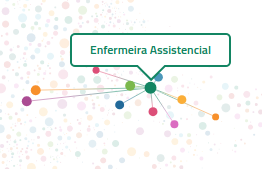
\includegraphics[scale=0.8, frame]{mapa-enfermeira-assistencial.png}
  \caption{Foco em uma ocupação}
  \source{Mapa de Carreiras}
  \label{fig:exemplo-grafo}
\end{figure}

% TODOS OS EXMPLOS DEVERIAM SER DA ÁREA QUE VAMOS ABORDAR, OU SEJA, TI. ISSO TRAZ MAIS DIDÁTICA E FOCO AO DOCUMENTO.

No contexto do Mapa de Carreiras, uma \textit{ocupação} significa uma atividade profissional, remunerada ou não. A maior parte dessas ocupações são profissões remuneradas, tais como \enquote{Babá} ou \enquote{Arquiteto}. Entretanto, algumas delas aparecem como atividade principal de uma pessoa, mas não são necessariamente uma profissão, tais como \enquote{Mestrando}, \enquote{Enfermeiranda} ou \enquote{Voluntário}. Os vértices possuem diversos atributos que são resumos estatísticos daquela ocupação, tais como a distribuição salarial, a distribuição do tempo de permanência em uma ocupação, entre outras.

% ENTÃO UM VÉRTICE NA VERDADE SERÁ UM VETOR DE CARACTERÍSTICAS COM ESSAS INFORMAÇÕES. PRECISAMOS DEFINIR EXATAMENTE QUAIS CARACTERÍSTICAS COMPORÃO O VETOR DE CARACTERÍSTICAS DOS VÉRTICES. Ronie: Coloco isso dentro da Metodologia?
% COLOQUE A DESCRIÇÃO (VETOR DE CARACTERÍSTICAS) DO VÉRTICE AQUI MESMO.

As arestas que conectam as ocupações representam \textit{movimentações} entre elas, ou seja, o fluxo de pessoas que exercia uma certa ocupação e passou a exercer outra. Acompanhar as arestas permite observar o movimento dos profissionais em suas carreiras. O peso das arestas é o número de profissionais que fizeram a trajetória de uma ocupação para outra. A figura~\ref{fig:exemplo-medico-do-trabalho} exibe as arestas a partir da ocupação \enquote{Médico do Trabalho} como exibidos pelo site do Mapa da Carreiras.

\begin{figure}[ht]
  \centering
  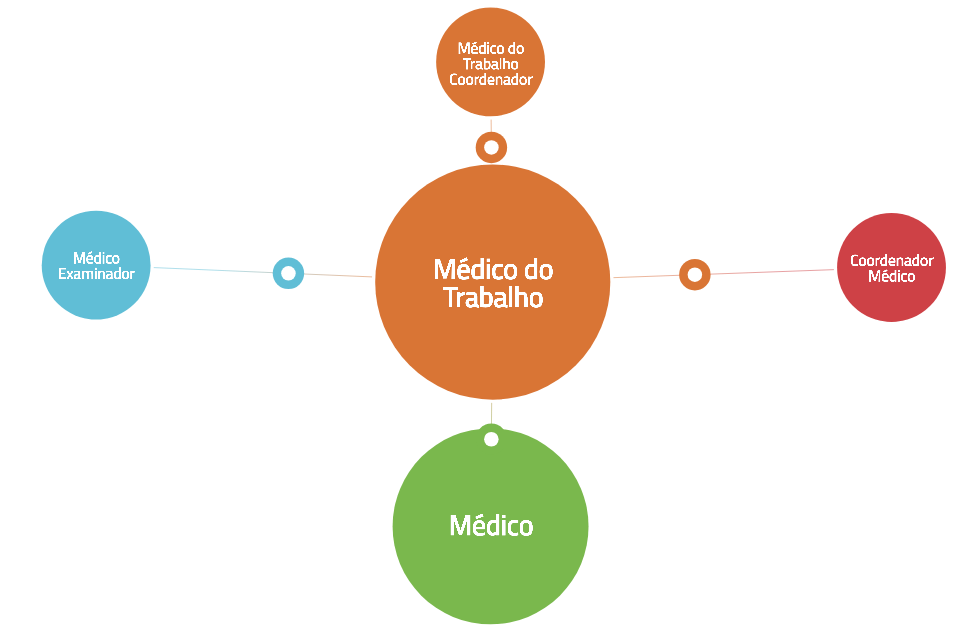
\includegraphics[scale=0.25]{mapa-medico-do-trabalho.png}
  \caption{Ocupações diretamente relacionadas a Médico do Trabalho}
  \source{Mapa de Carreiras}
  \label{fig:exemplo-medico-do-trabalho}
\end{figure}

% TODOS OS EXMPLOS DEVERIAM SER DA ÁREA QUE VAMOS ABORDAR, OU SEJA, TI. ISSO TRAZ MAIS DIDÁTICA E FOCO AO DOCUMENTO.

É importante esclarecer que a visualização observada no site do Mapa da Carreiras foi construída para permitir uma navegação simplificada para o usuário (ref). Para essa pesquisa, os dados utilizados são os mesmos, mas em formatos mais adequados ao projeto. Por exemplo, o equivalente da figura~\ref{fig:exemplo-medico-do-trabalho} utilizada para análise exploratória pode ser vista na figura~\ref{fig:grafo-medico-do-trabalho}. Nela, é possível observar ocupações que não estão diretamente relacionadas a \enquote{Médico do Trabalho}, mas que estão no mesmo agrupamento, como \enquote{Médico Plantonista}.

\begin{figure}[ht]
  \centering
  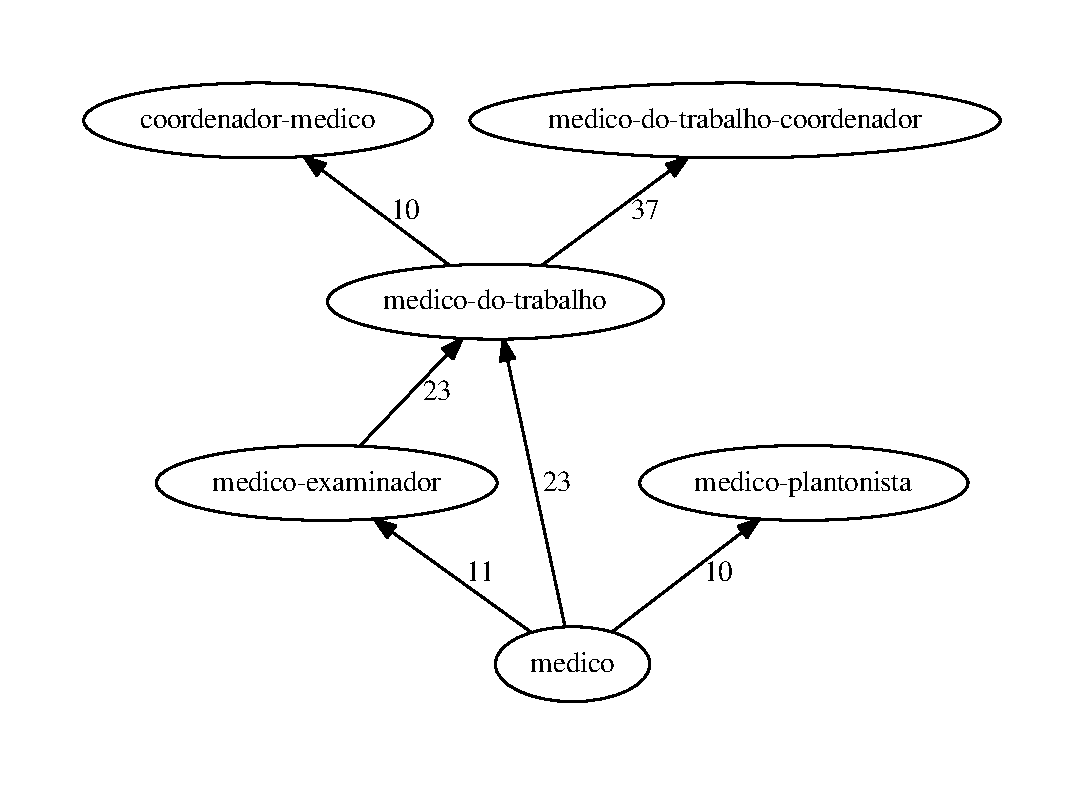
\includegraphics[scale=0.6]{cluster_24.pdf}
  \caption{Grafo ao redor de Médico do Trabalho}
  \source{Elaboração do autor}
  \label{fig:grafo-medico-do-trabalho}
\end{figure}

O grafo do MCar é direcionado e, portanto, o fluxo de profissionais entre ocupações possui uma direção específica, mas é comum que existam movimentações em ambos os sentidos entre duas ocupações. Esse movimento é representado por duas arestas diferentes, mesmo que no site ela seja representada por uma única aresta. Em outras palavras, o MCar é um grafo direcionado com ciclos, porém os vértices não são autorreferentes.

Por conta dos ciclos, não é possível criar uma ordenação topológica que represente uma clara progressão de carreira para o grafo como um todo. Entretanto, é possível extrair grupos de ocupações que possuem movimentações mais frequentes entre si. Esses agrupamentos são comumente acíclicos, o que possibilita traçar essa progressão entre as ocupações que o compõem. Nos experimentos do Capítulo XX é possível observar que essa característica é mais frequentemente observada em grupos formados por ocupações que requerem maior qualificação técnica, como \enquote{Comércio Exterior} ou \enquote{Médico do Trabalho}, como visto na figura~\ref{fig:grafo-medico-do-trabalho}. Já nas ocupações ditas \enquote{operacionais}, o fluxo de movimentação entre ocupações acentua a característica cíclica do grafo. Particularmente, é possível observar um forte ciclo entre as ocupações \enquote{Recepcionista}, \enquote{Vendedor} e \enquote{Auxiliar Administrativo}, como mostrado pela figura~\ref{fig:grafo-ciclo-operacional}.

\begin{figure}[ht]
  \centering
  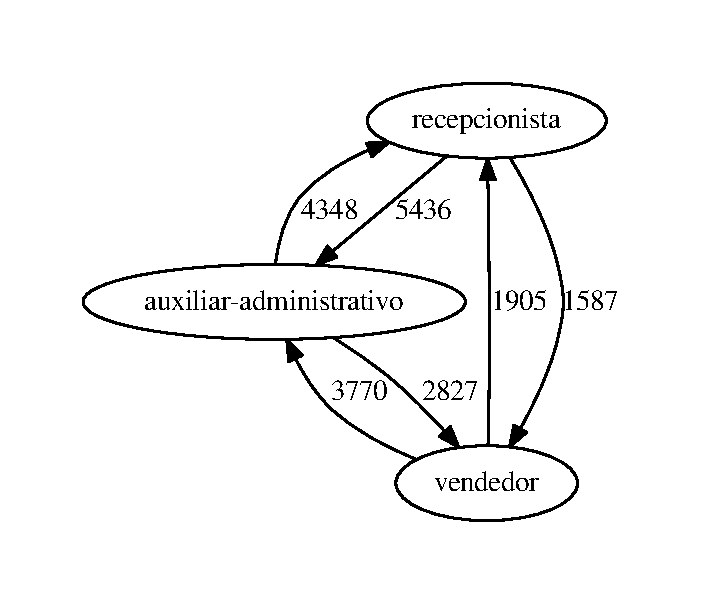
\includegraphics[scale=0.8]{ciclo-operacional.pdf}
  \caption{Ciclo entre Ocupações}
  \source{Elaboração do autor}
  \label{fig:grafo-ciclo-operacional}
\end{figure}

Para a construção dos vértices, os textos presentes nos títulos dos históricos profissionais dos currículos foram \enquote{normalizados}. Nesse contexto, \enquote{normalização} significa transformar os títulos com o mesmo significado na mesma representação textual. Por exemplo, a mesma ocupação pode ter sido registrada por pessoas diferentes como \enquote{Moto Boy}, \enquote{moto boy}, \enquote{Motoboy}, \enquote{Moto Girl} entre outras variações. O que chamamos de \enquote{normalização} é o trabalho de transformar essas diferentes grafias em uma única classe que possa ser usada para identificação da ocupação. No caso, todas as anteriores são normalizadas para \enquote{motoboy}. Esse trabalho também inclui a correção ortográfica e a remoção de abreviação das ocupações.

Após a normalização são criados pares de ocupações cronologicamente ordenados. Isso significa que o término de uma ocupação precisa coincidir com o início da seguinte. Uma margem de dois meses de tolerância na sobreposição corrige pequenas imprecisões na anotação dos históricos profissionais. Currículos com apenas uma ocupação são descartados, bem como ocupações que se sobreponham cronologicamente ou que estejam separadas por um intervalo de tempo maior que um ano.

Os pares de ocupações são unificados produzindo as arestas e os vértices, e as arestas menos relevantes do grafo, ou seja, aquelas com menos de dez movimentações, são podadas. Esse critério de poda foi definido empiricamente através de análise por amostragem. Números muito maiores removem vértices de ocupações mais especializadas como \enquote{Comandante} ou \enquote{Engenheiro de Minas}, enquanto números muito menores acrescentavam vértices espúrios causados por erros de grafia que a fase de correção ortográfica foi incapaz de detectar.

Um dos efeitos indesejados desse processo é que algumas ocupações legítimas são removidas do grafo. É o caso de ocupações muito recentes, muito especializadas, ou que ainda não possuem uma concordância da nomenclatura entre os profissionais da área. Como exemplo podemos citar \enquote{Especialista em Experiência do Usuário}, uma profissão recente, que também é chamada \enquote{Analista de UX} ou apenas \enquote{UX}.

% NÃO DEVERÍAMOS CRIAR UM DICIONÁRIO DE EQUIVALÊNCIA DE NOMENCLATURA E SUBTITUIR AS MÚLTIPLAS NOMENCLATURAS POR UMA PADRÃO?
% Ronie: Dá até para fazer manualmente, mas resisto a isso. O motivo pode ser exemplificado pelas ocupações "Analista de Inteligência de Negócios"  e "Analista de BI (Business Intelligence)", apenas o termo traduzido ou um estrangeirismo, entretanto analisando a nuvem de palavras é possível ver que são funções bem diferentes. E olha que é da nossa área e deveríamos saber disso >_<
% Links abaixo:
% http://www.vagas.com.br/mapa-de-carreiras/cargos/analista-de-bi/0
% http://www.vagas.com.br/mapa-de-carreiras/cargos/analista-de-inteligencia-de-negocios/0

Duas outras limitações no grafo ocorrem por conta da experiência profissional ser um campo de texto livre, ou seja, o usuário digita livremente sua ocupação sem estar restrito a uma lista de opções. A primeira se refere a ocupações que foram digitadas para representar uma ocupação dupla, como \enquote{Caixa e Balconista} ou \enquote{Atendente/Estoquista}. A segunda ocorre por ambiguidade no nome da ocupação, como \enquote{Coordenador de Projetos}, que ocorre na carreira de Desenvolvimento de Software e na de Engenharia Civil.

Por outro lado, o campo de texto livre permite a captura de ocupações que pouco provavelmente apareceriam em uma lista curada, como \enquote{IRLA} (Instalador Reparador de Linhas Aéreas) ou \enquote{Rigger} (pessoa no solo que orienta o posicionamento de carga para o operador de guindaste).

Ao final do processo o grafo possui cerca de 8.348 ocupações distintas e 14.031 arestas. Esses números flutuam dependendo das atualizações dos currículos em que são baseados e no crescimento natural do banco de dados. Os dados utilizados nesse trabalho refletem a base atualizada em Fevereiro de 2017.


\subsection{O Processo de Construção do Mapa de Carreiras} \label{sec:construcao}

O Mapa de Carreiras é construído a partir dos currículos de um banco relacional condensando seus dados para formar um grafo de movimentação de pessoas entre as ocupações.
% AQUI NA INTRODUÇÃO SUGIRO COLOCAR UM FLUXOGRAMA COM OS BLOCOS DE CONSTRUÇÃO DO MCAR. NA LINHA ABAIXO MENCIONE QUE CADA SEÇÃO VAI DESCREVER UM BLOCO DO PROCESSO.

As seções a seguir descrevem os passos envolvidos na montagem do grafo.

\subsubsection{Os Dados}

Os dados fonte para essa pesquisa são currículos anonimizados de usuários do site de carreiras VAGAS.com.br. Esses currículos são armazenados em um banco de dados \textit{Microsoft SQL Server}. No total há cerca de 10 milhões de currículos~\todo{Colocar número exato} armazenados entre 1999 e 2016, mas para esse trabalho apenas os currículos atualizados entre 2011 e 2016 são utilizados~\todo{Colocar número exato}.

% FALE AGORA DOS CVS DA ÁREA DE TECNOLOGIA. QUANTOS SÃO? QUANTAS E QUAIS SÃO AS CARREIRAS (A LISTAGEM DAS CARREIRAS PODE VIR COMO UM APÊNDICE)
% Ronie: Focamos ainda na área de tecnologia? Acredito que poderíamos focá-la nos exemplos de carreiras maiores (como análise das redes livre de escala e mundo pequeno) que não são boas com carreiras muito pequenas como as que usei acima para exemplificar alguns grafos. Que acha?
% CONTINUO SUGERINDO PELO MENOS COMEÇARMOS COM A ÁREA DE TECNOLOGIA E, SE FOR O CASO, AMPLIAMOS DEPOIS.

Para as análises a serem explicadas nesse capítulo, os dados são primeiramente extraídos para arquivos texto e só então processados. Existem dois formatos usados nesse trabalho. O primeiro formato é descrito por \citeonline{Van_Dongen2008-kx} como \enquote{formato ABC}. Cada linha representa uma aresta, e cada aresta possui três campos separados por um ou mais espaços. Em um grafo direcionado, o primeiro campo é a aresta de partida, o segundo é a aresta de chegada e o campo final representa o peso da aresta. No caso do MCar, o peso representa o número de pessoas que se movimentou de uma ocupação à outra. Esse formato é usado na separação de carreiras através da \textit{clusterização} do grafo usando o \textit{Markov Clustering Algorithm} (MCL)~\cite{Van_Dongen2000-qm} e na montagem de visualizações exploratórias usando o programa \enquote{Graphviz}~\cite{Gansner2000-oo}.

\noindent\begin{minipage}{\linewidth}
\begin{lstlisting}[frame=single,caption=Arquivo em Formato ABC,label=lst:formato-abc,captionpos=b]
medico-examinador medico-do-trabalho 23
medico-do-trabalho coordenador-medico 10
medico-do-trabalho medico-do-trabalho-coordenador 37
medico medico-plantonista 10
medico medico-examinador 11
medico medico-do-trabalho 23
\end{lstlisting}
\end{minipage}

O segundo formato é uma lista de registros onde cada um ocupa uma única linha. Cada registro é codificado como uma \textit{array} de atributos no formato JSON (\textit{Javascript Object Notation}). Esse formato é usado em várias etapas da montagem do MCar e seu conteúdo varia de etapa para etapa. Os campos relevantes são descritos nas respectivas seções a seguir.

\subsubsection{O Processamento da Informação}

O volume de dados e a variedade de análises desse trabalho impõe algumas restrições de ordem prática que precisam ser contornadas. O volume de dados é grande o suficiente para exceder a memória de um computador convencional, algumas das ferramentas utilizadas não se comunicam com outras exceto através de arquivos texto e o tempo para processamento facilmente excede alguns dias se os processadores não forem adequadamente utilizados.

Essas restrições e a necessidade de atualizar continuamente os dados do MCar levaram a implementação de um sistema que executasse todos os passos para sua montagem de maneira automática.

A informação é processada em uma série de etapas consecutivas usando um padrão arquitetural conhecido como \textit{Dataflow}~\cite{Carkci2014-jk, Hohpe2003-nj}, especificamente o modelo conhecido como \textit{Pipes and Filters} ou \textit{Pipeline}. Nesse padrão, os dados fluem continuamente de um processo para o outro, sendo transformados e filtrados conforme o processo avança. 

Em uma estrutura de \textit{pipeline}, com exceção de alguns componentes especiais, cada processo possui apenas uma interface de entrada e uma interface de saída. Desde que mantenha a mesma interface, um processo pode ser substituído por outro, ou por um conjunto deles, sem afetar outras partes do sistema.

Essa arquitetura foi implementada em máquinas \textit{Linux} utilizando \textit{pipes} e \textit{sockets} para comunicação interprocessos. Um \textit{pipe} no \textit{Linux} é uma implementação de FIFO em memória RAM. A interface para \textit{push} na fila é idêntica a gravação de uma linha de texto em um arquivo. Do outro lado um outro processo lê a fila com a mesma interface de leitura de um arquivo linha a linha. Por usar interfaces compatíveis que leituras e gravações em arquivo, qualquer programa capaz de executar essas operações pode ser usado como parte do \textit{pipeline}. Isso resolve o problema do uso de ferramentas díspares, desde que sejam capazes de gravar e ler em arquivos texto, são capazes de se integrar ao processo como um todo.

Enquanto \textit{pipes} permitem a comunicação interprocessos na mesma máquina, \textit{sockets} podem ser usados para comunicação entre computadores através de uma interface padronizada. Ao invés dos \textit{sockets} nativos do \textit{Linux}, optou-se pelo \textit{ZeroMQ} que é uma implementação mais robusta, criada para transmitir dados usando diversos modelos de distribuição~\cite{Hintjens2013-tz}.

O \textit{ZeroMQ} possui interfaces para diversas linguagens de programação, mas para preservar a interface entre processos foram criados componentes que traduzem a entrada em \textit{pipes} para \textit{sockets ZeroMQ} e vice-versa. Em termos práticos, a comunicação entre processos pode ser feita entre processos da mesma máquina ou entre diferentes computadores de maneira transparente.

A maior parte dos processos foi implementada usando a linguagem Ruby, mas alguns processos foram implementados usando Python ou programas específicos, como o MCL para \textit{clusterização} e o Graphviz para posicionamento do grafo em um plano bidimensional.

A montagem do grafo é mostrada na figura~\ref{fig:montagem-do-grafo}.

\begin{figure}[ht]
  \centering
  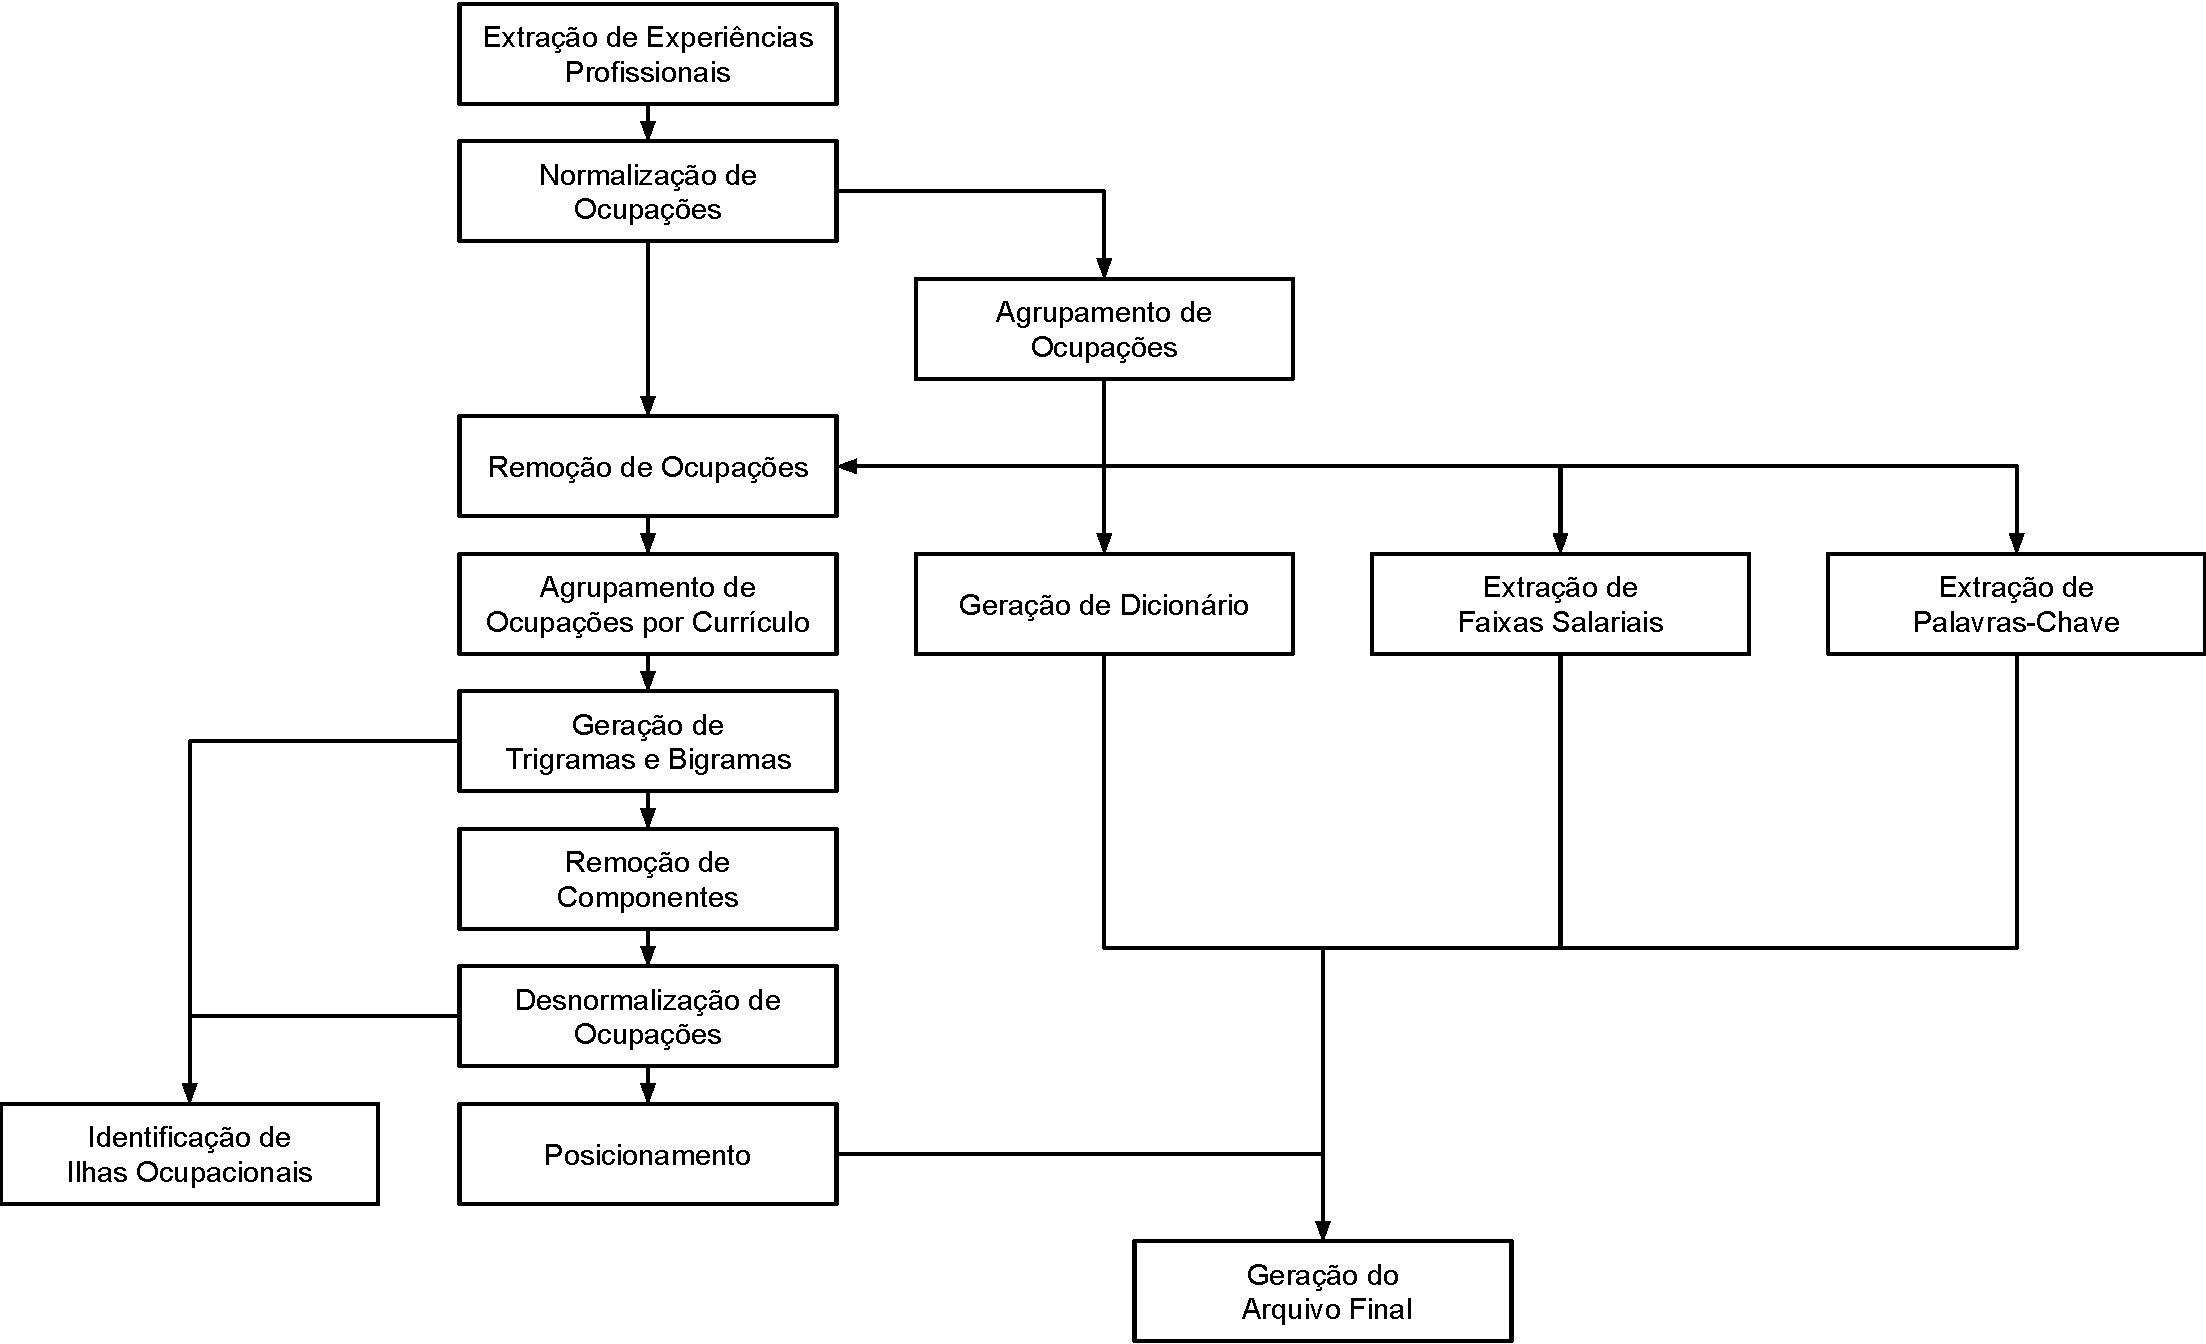
\includegraphics[scale=0.4]{pipeline1.pdf}
  \caption{Montagem do Grafo}
  \label{fig:montagem-do-grafo}
\end{figure}

\subsubsection{Extração do Experiências Profissionais} \label{sec:extracao-experiencia}

O primeiro processo do \textit{pipeline} extrai os registros do bancos de dados relacional e os grava em arquivos texto. O processo não extrai currículos, mas sim experiências profissionais. Cada registro representa uma única experiência.

Os dados extraídos são:

\begin{description}

  \item[Identificador do Currículo] é um número único para cada currículo dentro do banco de dados. Ele é usado posteriormente para agrupar as experiências profissionais por pessoa.

  \item[Nome da Ocupação] é o texto digitado livremente pelo usuário no campo nomeado \enquote{Cargo} no currículo. Esse texto dá origem aos nomes das ocupações usadas no Mapa de Carreiras.

  \item[Data de Início] e \textbf{Data de Término} marcam quando o profissional iniciou naquela ocupação e até quando a exerceu. Se é a ocupação atual, não existe uma data de término. Esses campos são usados para determinar a sequência de experiências profissionais que formarão as arestas do grafo.

  \item[Texto Descritivo] é o texto digitado livremente pelo usuário no campo com o nome \enquote{Descrição} no currículo. Esse campo é usado para criar uma nuvem de palavras-chave sobre a ocupação.

\end{description}

\subsubsection{Normalização de Ocupações} \label{sec:normalizacao}

Nessa etapa, o nome da ocupação é normalizado para uma classe de maneira que todas as grafias significando a mesma ocupação sejam transformadas em uma mesma classe. Nessa pesquisa a classe é chamada \enquote{classe equivalente} ou \enquote{ocupação normalizada}.

Para transformar o texto digitado em uma ocupação normalizada os erros de digitação são corrigidos, pontuações são removidas, abreviaturas frequentes são expandidas, o texto é colocado em minúsculas, é feita a singularização das palavras que compõem a ocupação e os nomes são masculinizados (\enquote{secretária} se transforma em \enquote{secretário}, por exemplo).

Ocupações com múltiplas palavras também são ordenadas alfabeticamente. Dessa forma, ocupações como \enquote{Auxiliar Financeiro-Administrativo} e \enquote{Auxiliar Administrativo-Financeiro} resultam na classe \enquote{administrativo auxiliar financeiro}.

As classes resultantes lembram vagamente o termo original, como no exemplo acima. No processo descrito na seção~\ref{sec:criar-dicionario}, é criado um dicionário entre a classe equivalente e um nome que tenha significado para o usuário.

\subsubsection{Remoção de Ocupações Incorretas} \label{sec:remocao-ocupacoes-incorretas}

Mesmo após a remoção de casos únicos, alguns nomes presentes nesse campo não podem ser realmente considerados ocupações. São erros comuns que a etapa de normalização não é capaz de corrigir ou representam um entendimento equivocado por parte do usuário.

Casos emblemáticos são os textos \enquote{sim}, \enquote{não} ou \enquote{o mesmo} encontrados no campo destinado ao nome da ocupação. A remoção desses casos precisou ser feita manualmente, ou seja, especialistas da empresa revisaram a lista de ocupações e criaram um dicionário com os erros mais comuns utilizados nessa etapa do processo. Esse dicionário foi aprimorado com sugestões dos usuários após a publicação do MCar.

\subsubsection{Agrupamento de Ocupações por Currículo}

As ocupações são agrupadas por currículo, formando uma sequência cronológica das experiências de um profissional. Até essa etapa, há uma experiência profissional por registro, após ela, cada registro contém uma sequência de experiências profissionais do mesmo indivíduo, ordenadas cronologicamente.

% Inserir um diagrama com os campos. Ronie 2017-04-30

\subsubsection{Remoção de Experiências sem Conexão ou Sobrepostas}

Como o objetivo final é criar um grafo que sumarize o \textit{movimento} de pessoas entre ocupações, as experiências profissionais que não se conectam cronologicamente com nenhuma outra são removidas. Serão consideradas desconexas quaisquer experiências em sequência cujo início da posterior esteja a mais do dois meses de distância do fim da anterior.

% Inserir um gráfico explicativo. Ronie 2017-02-30

Na mesma etapa, removem-se experiências profissionais que se sobreponham. Uma vez sobrepostas, não é possível afirmar que uma é sequência natural da outra ou que sequer tenham relação entre si. É comum encontrar no banco de dados carreiras paralelas em que gestores também são professores ou técnicos que também sejam voluntários. Da mesma maneira que experiências desconexas, as que se sobrepõem por mais de dois meses são removidas.

\subsubsection{Remoção de Currículos por Experiência}

Após o processo anterior, são removidos os registros que possuam apenas uma ou nenhuma experiência profissional.

\subsubsection{Geração de Pares de Experiência}

As experiências profissionais de cada currículo são pareadas por ordem cronológica. Por exemplo, um currículo que tenha a seguinte sequência de ocupações \enquote{Faxineiro \textrightarrow~Copeiro \textrightarrow~Chapeiro}, produz os pares \enquote{Faxineiro \textrightarrow~Copeiro} e \enquote{Copeiro \textrightarrow~Chapeiro}.

Antes desse processo, cada registro é uma sequência de experiências profissionais. O processo expande cada registro em múltiplos registros, cada um representando um par de experiências profissionais de um único indivíduo.

\subsubsection{Agrupamento de Pares de Ocupações}

Pares iguais de ocupações são agrupados e contados, gerando um \textit{multiset}, ou seja, um conjunto com o número de repetições de cada elemento. O número de repetições em um par representa o número de pessoas que se movimentaram de uma ocupação para outra.

As etapas posteriores podam o grafo em suas arestas menos relevantes e transformam sua representação textual para que possa ser lido por outros programas.

\subsubsection{Remoção de Pares Pouco Frequentes} \label{sec:grafo-final}

A maioria dos pares de ocupações ocorrem pouquíssimas vezes. Em um conjunto com XX pares, cerca de XX ocorrem apenas uma vez. Esse pequeno número de repetições é causado tanto por trajetórias incomuns, quanto por erros de digitação que as etapas anteriores não foram capazes de eliminar. Por vezes são apenas ocupações similares a outras, mas onde os usuários escrevem de maneira pouco convencional. Com alguma frequência, os pares realmente representam trajetórias em carreiras extremamente específicas.

Para encontrar um número de corte foi feita uma avaliação manual por amostragem. Amostras com algumas centenas de pares com números de corte entre 1 e 30 foram analisadas por especialistas da empresa junto com o pesquisador. O objetivo foi encontrar um número que não fosse conservador demais, removendo trajetórias válidas, nem liberal demais, permitindo trajetórias com erro.

Após o processo de análise, chegou-se a um número próximo a 10 repetições. Pares de ocupações com menos de 10 repetições são removidos.

A partir desse ponto, os dados para a montagem do grafo estão prontos em formato texto.

\subsubsection{Posicionamento dos Vértices do Grafo}

Para que o grafo possa ser exibido bidimensionalmente, é preciso que seus vértices sejam posicionados de modo a evitar a sobreposição e que os vértices relacionados por arestas de maior peso estejam mais próximos.

O algoritmo de \textit{Force-Directed} (ref) é usado para posicioná-los corretamente. Esse algoritmo é aplicado nesse passo utilizando o programa Graphviz. A saída do Graphviz é um arquivo texto com a posição X e Y do vértice em um plano cartesiano.

\subsubsection{Descoberta de Proto-Carreiras}

%% O QUE É UMA PROTO-CARREIRA?

% Me parece que "proto-carreiras" não é um nome lá muito bom, mas foi o que consegui por enquanto =/ Ronie 2017-04-29
% Aqui também tem uma dose não saudável de especulação baseado no tempo que fiquei olhando para esse grafo. Pode ser o caso de colocar números em tudo (gosto disso), ou eliminar boa parte do texto. Ronie 2017-04-30

O grafo gerado no passo~\ref{sec:grafo-final} é usado nesse processo para gerar agrupamentos.

Entre duas ocupações o maior fluxo de movimentações indica uma certa preferência por uma das duas. Por exemplo, se o número de movimentações entre \enquote{Analista de Sistemas \textrightarrow~Coordenador de Projeto} for maior que o reverso \enquote{Coordenador de Projeto \textrightarrow~Analista da Sistemas}, considera-se que \enquote{Coordenador de Projeto} é uma ocupação que sucede \enquote{Analista de Sistemas}. Algumas vezes o fluxo entre as ocupações é tão similar que não é possível dizer que há uma ordem de sucessão, como no caso apresentado no ciclo de ocupações operacionais na figura~\ref{fig:grafo-ciclo-operacional}; em outros, o sentido contrário possui um fluxo várias vezes menor ou não há fluxo contrário, como o caso do grafo sobre \enquote{Médico do Trabalho} na figura~\ref{fig:grafo-medico-do-trabalho}.

\todo[inline]{Ronie: estou pensando que a seção abaixo pode ser movida para \enquote{conclusões} ou mais para frente, que acha?}

Quando o fluxo de pessoas de uma ocupação para outra é relevante, é possível notar que essa ordem de preferência vai normalmente de ocupações mais operacionais e com salários mais baixos para ocupações mais gerenciais e com salários mais altos. Isso coincide com a senso comum de progressão de carreira.

A grosso modo, o agrupamento e o fluxo de migração das ocupações revela o que se pode considerar um \enquote{protótipo de carreira}. Ou seja, um esboço onde um indivíduo em uma ocupação dentro desse grupo tem uma probabilidade maior de se manter nele e de se movimentar para ocupações no topo do grupo.

Existe, no entanto, um grupo que não obedece às características descritas acima. Ao se tentar ordená-lo topologicamente, não há uma ordem de preferência clara entre as ocupações, o que indica que não há uma noção de sucessão como em outros grupos, como exemplificado anteriormente na figura~\ref{fig:grafo-ciclo-operacional}. Ele também possui algumas ocupações que conectam uma grande quantidade de outras ocupações, como \enquote{Auxiliar Administrativo}, que possui movimentações com XX ocupações, cerca de XX\% das ocupações do MCar.

Ao analisar o grupo, nota-se que a escolaridade mais frequente nessas ocupações é a de \enquote{segundo grau completo}, significando que essas ocupações não necessitam de treinamento especializado para serem desempenhadas, o que é um indício que esse grupo reflete a própria definição de \enquote{operacional}.

Algumas outras ocupações também possuem \enquote{segundo grau completo} como escolaridade mais frequente, mas se comportam como os grupos com uma direção clara de preferência entre as ocupações. Uma análise manual da descrição das suas ocupações e das palavras-chave relacionadas sugere que essas são ocupações \enquote{técnicas}. Ou seja, uma ocupação que requer um treinamento não-trivial, mas não tão exigente quanto uma graduação. Como exemplo, é possível observar a carreira de cozinheiro na figura~\ref{fig:exemplo-grafo-cozinheiro}.

\begin{figure}[htb]
  \centering
  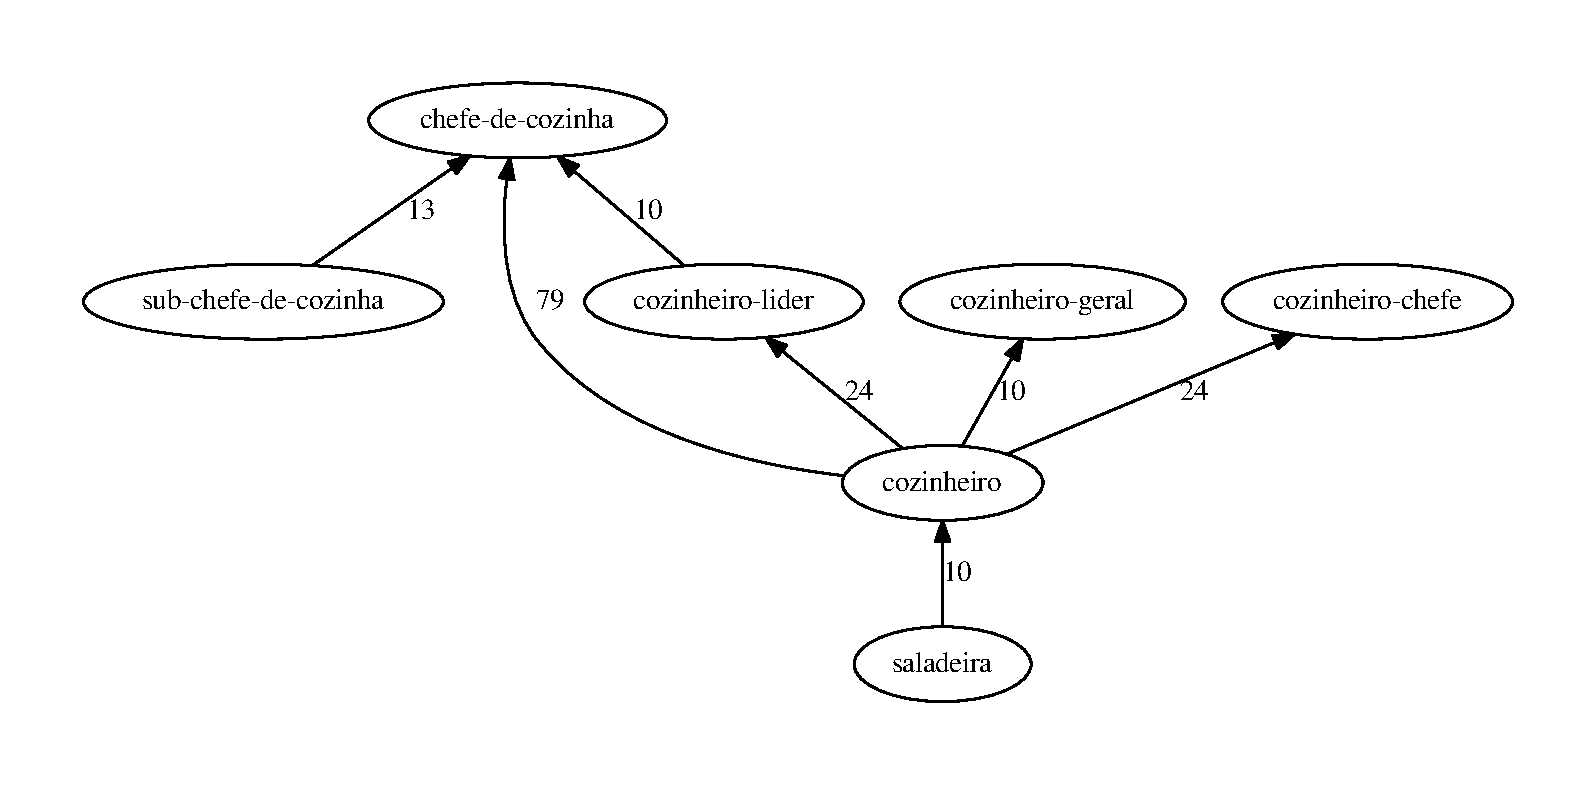
\includegraphics[scale=0.6]{subcluster_01_11.pdf}
  \caption{Carreira Técnica de Cozinheiro}
  \label{fig:exemplo-grafo-cozinheiro}
\end{figure}

\subsubsection{Agrupamento de Ocupações}

Esse processo agrupa os dados gerados pelo processo descrito na seção\ref{sec:remocao-ocupacoes-incorretas} por ocupação. Cada ocupação normalizada agora possui uma lista com suas grafias originais, uma lista com as descrições daquela experiência profissional escrita por cada indivíduo, bem como a quantidade de ocupações agrupadas.

\subsubsection{Remoção de Ocupações com Pouca Frequência}

Mesmo com o processo de correção e normalização, algumas experiências profissionais são escritas de maneira única. Isso pode significar um erro, uma ocupação singular ou o uso de termos pouco convencionais. Como o objetivo da montagem do grafo é extrair as carreiras mais frequentes, os casos únicos podem ser seguramente removidos sem a necessidade de determinar sua causa.

\subsubsection{Criação de Dicionário para Exibição} \label{sec:criar-dicionario}

Os textos resultantes do processo de normalização descrito na seção~\ref{sec:normalizacao} não são adequados para exibição. Esse processo contabiliza o número de grafias exatamente idênticas para cada ocupação normalizada e assume como \enquote{nome de exibição} a grafia mais frequente.

A limitação desse processo é que algumas ocupações são descritas no masculino ou no feminino dependendo do número de profissionais do gênero exercendo esse ocupação. Por exemplo, uma das ocupações de Direito é descrita como \enquote{Advogado} (no masculino) pois existem um pouco mais profissionais do gênero masculino exercendo a profissão, por outro lado, outra ocupação correlacionada é descrita como \enquote{Advogada Coordenadora} pelo motivo contrário.

Apesar da regra da língua portuguesa do uso do masculino quando há um grupo de gênero misto (ref), optou-se por não se modificar o gênero artificialmente, preservando a grafia da predominância do gênero na ocupação.

\subsubsection{Extração de Palavras-Chave}

As palavras-chave são extraídas a partir das descrições digitadas pelos usuários no campo \enquote{Experiência Profissional} dos currículos. O processo descrito abaixo tenta criar expressões significativas, ou seja, pequenas frases, que ajudem a descrever o cargo ao invés de apenas indicar as palavras mais comuns. Um fato notável é que não é possível utilizar \textit{stemming} ou correção ortográfica nesse processo, pois existe uma grande quantidade de jargões e siglas específicos nas descrições.

Para formar expressões, são gerados unigramas, bigramas e trigramas para as descrições de cada experiência profissional. A seguir, elas são ordenadas por TF-IDF e as palavras que aparecem repetidas em um n-grama de menor TF-IDF são removidas. Por exemplo, se a palavra \enquote{fiscal} aparece com maior TF-IDF que o bigrama \enquote{nota fiscal}, a palavra \enquote{fiscal} é removida da lista.

% Ronie: na prática, o resultado é muito bom, mas o algoritmo foi baseado no meu nariz =/ Então, talvez eu devesse refazer o processo com uma técnica de sumarização melhor.

\subsubsection{Gravação do Arquivo Final}

A definir\ldots

\subsection{Atributos das Ocupações}

Complementar à montagem do grafo, os vértices com as ocupações são abastecidos com outras informações. São elas:

\begin{description}
  \item[Idade] computada para cada ocupação considerando a data de nascimento do profissional e a data de entrada na ocupação.
  \item[Salário] da ocupação atual corrigido pelo IPCA a partir da última data de atualização do currículo.
  \item[Tempo de Permanência na Ocupação] extraída a partir do número de meses consecutivos do indivíduo naquela experiência profissional.
  \item[Escolaridade] registrada no currículo com as opções 1º, 2º e 3º graus completos.
  \item[Curso de Graduação] registrada a partir de uma lista de cursos, essa informação é coletada apenas para escolaridade acima de 2º grau completo. A graduação é considerada apenas para as ocupações que ocorrem depois do término do curso.
  \item[Gênero] do profissional, apenas masculino ou feminino.
  \item[Número de Profissionais na Ocupação] é obtido contando as ocupações que não possuem data de término.
\end{description}

A idade, o salário e o tempo de permanência são sumarizados usando o \textit{resumo de cinco números}, com seus intervalos de confiança 95\% e uma \textit{estimativa de densidade de probabilidade}. Já a escolaridade, o curso de graduação e o gênero são simples contagens de frequência.

O \textit{resumo de cinco números} consiste no valor mínimo, 1º quartil, mediana, 3º quartil e valor máximo. Esse resumo é proposto por \citeonline{Hoaglin1983-aq} como estatística descritiva de uma amostra.

O intervalo de confiança 95\% para todos os valores do resumo de cinco números é obtido por \textit{bootstrap} com 10.000 iterações. A técnica permite identificar os valores mais confiáveis independentemente do tamanho da amostra e das distribuições. A tabela~\ref{tab:resumo-salario-programador} mostra o resumo e seus intervalos de confiança para a ocupação de \enquote{Programador}.

\begin{table}[htb]
\centering
\begin{tabular}{r|c|c|c}
                    & \textbf{2,5\%} & \textbf{Estimativa} & \textbf{97,5\%} \\ \hline
\textbf{Mínimo}     & [coletar]      & [coletar]           & [coletar] \\ \hline
\textbf{1º Quartil} & 1672           & 1709                & 1751 \\ \hline
\textbf{Mediana}    & 2354           & 2403                & 2476 \\ \hline
\textbf{3º Quartil} & 3225           & 3294                & 3354 \\ \hline
\textbf{Máximo}     & [coletar]      & [coletar]           & [coletar]    
\end{tabular}
\caption{Resumo de 5 números para salário de \enquote{Programador}}
\label{tab:resumo-salario-programador}
\end{table}

A \textit{estimativa de densidade de probabilidade} é obtida por um Estimador de Densidade de Kernel usando um distribuição gaussiana como função kernel. A largura de banda escolhida para cada estimativa é o menor valor limite para que a distribuição se mantenha unimodal.

\section{HIPÓTESES}

\todo[inline]{Título provisório}

Aqui estão as hipóteses para o MCar baseadas nas métricas de rede.

\begin{hypothesis}[Atração Profissional]
A força de entrada no nó significa o quanto uma ocupação atrai profissionais. Nós de grande força de entrada funcionam como polos atratores de mão de obra, seja pela demanda, seja pela facilidade em exercer a ocupação ou por sua atratividade.
\end{hypothesis}
%% ACHEI ESSA COLOCAÇÃO MUITO INTERESSANTE. UMA VEZ VALIDADA QUANTITATIVAMENTE É UMA OBSERVAÇÃO IMPORTANTE PARA SER COLOCADA EM UMA CONCLUSÃO OU ANÁLISE DE RESULTADOS

\todo[inline]{Verificar e checar duplamente a correlação}

\begin{hypothesis}[Correlação Negativa entre a Força de Entrada e a Mediana Salarial]
Existe uma correlação negativa entre a força de entrada e a mediana salarial, ou seja, quanto maior a força, menor a mediana do salário.
\end{hypothesis}

Essa correlação é consistente com o conceito de \textbf{mercado de trabalho} em que quanto maior a oferta de mão de obra, menor o salário pago. Entretanto, não é possível afirmar que existe um excesso de profissionais para uma certa ocupação, pois nesse trabalho não foi possível medir se a ocupação está \textit{saturada}. 
%% MINHA LEITURA É UM POUCO DIFERENTE. COMO O GRAFO É CONSTRUÍDO A PARTIR DE DADOS REAIS, QUANTO MAIOR A FORÇA DE ENTRADA, MAIS PROFISSIONAIS CONVERGEM PARA ESSA PROFISSÃO E, NORMALMENTE, AS PROFISSÕES QUE POSSUEM MAIORES SALÁRIOS SÃO AQUELAS QUE TÊM MENOS PESSOAS, POIS ESTÃO MAIS NO TOPO DA PIRÂMIDE. PORTANTO, EU ENTENDO QUE A OFERTA DE MÃO DE OBRA É UM ELEMENTO IMPORTANTE, MAS TAMBÉM DEVEMOS CONSIDERAR AS HABILIDADES REQUERIDAS PARA A POSIÇÃO.
% Ronie: Sim, essa é uma discussão muito boa! Eu gostaria de me aprofundar mais nela se houver tempo hábil.

Por outro lado, é possível observar na lista XX que essas ocupações coincidem intuitivamente com as noções de \enquote{início de carreira} e \enquote{ocupação operacional}.

\begin{hypothesis}[Pontos de Saída do Mercado de Trabalho]
Se $\linkin{s}_i \gg \linkout{s}_i$, a movimentação não mapeada não é suficiente para explicar a diferença entre as forças, o que possivelmente indica que os profissionais estão de fato se acumulando durante os anos, sugerindo que esse nó é um ponto de saída do mercado de trabalho.
\end{hypothesis}

\begin{hypothesis}[Pontos de Entrada do Mercado de Trabalho]
De maneira análoga, as ocupações em que $\linkin{s}_i \ll \linkout{s}_i$ indicam ocupações que são entrada para o mercado de trabalho.
\end{hypothesis}

\begin{hypothesis}[Trabalho de Passagem]
Uma ocupação com alta intermediação significa um \enquote{trabalho de passagem}, em que um grande fluxo de profissionais passa por ela a caminho de outros trabalhos.
\end{hypothesis}

\todo[inline]{Não é bem isso que eu quero dizer, mas não estou achando a ideia correta. No que observei até agora, as carreiras normalmente afunilam em um cargo e depois abrem para o topo, é obviamente um ponto de crítico, mas estou com dificuldade de elaborá-lo.}

A Figura~\ref{fig:carreira-topografia} ilustra o conceito na carreira de topografia, onde o nó em destaque representa a ocupação com maior centralidade de intermediação.

\begin{figure}[ht]
  \centering
  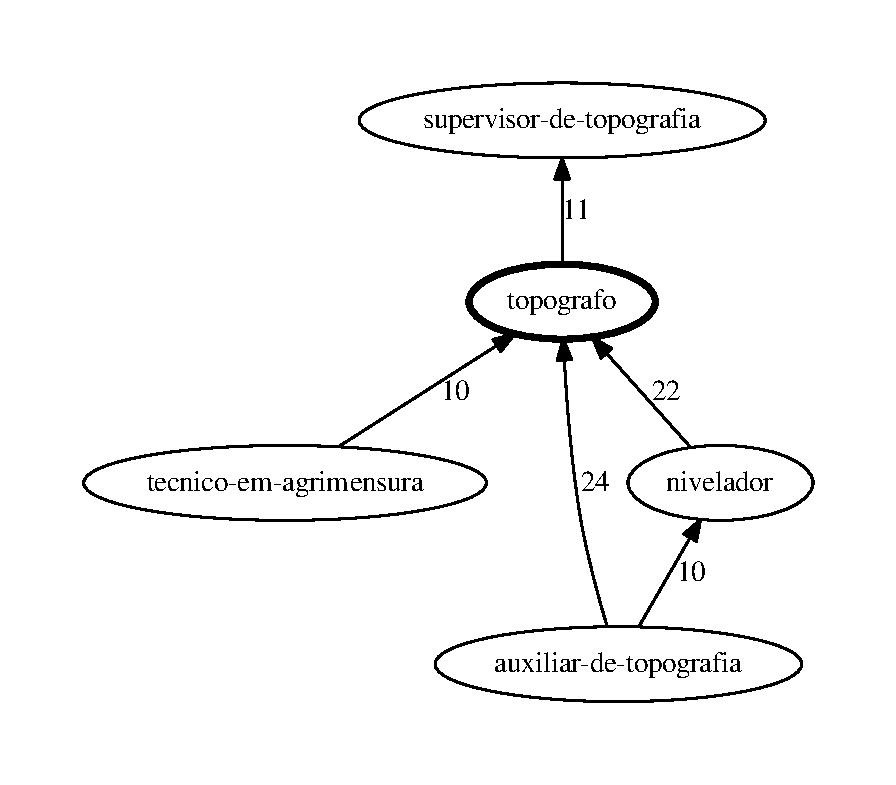
\includegraphics[scale=0.6]{cluster_25.pdf}
  \caption{Ilustração da centralidade de intermediação na carreira de topografia. O nó mais central é o "topógrafo".}
  \label{fig:carreira-topografia}
\end{figure}

\begin{hypothesis}[Equivalência Profissional] \label{hip:equivalencia}
Em uma análise local, se $\recout{w}_{ij}$ é próximo de zero, ou se $\recout{w}_{ij} \ll \recboth{w}_{ij}$, significa que não há um sentido de \enquote{progressão} entre uma ocupação e outra, ou seja, profissionais vão e vêm entre elas sem uma preferência óbvia no fluxo, indicando que são equivalentes em termos profissionais.
\end{hypothesis}

Ao se analisar a reciprocidade global $\weighted{\rho}$ em componentes do MCar extraídos por agrupamento, é possível observar características de reciprocidade bastante distintas. Enquanto alguns componentes possuem alta reciprocidade, outros são claramente anti-recíprocos, sugerindo que há um caminho claro para os profissionais que se encontram naquele componente.

\begin{hypothesis}[Inferência de Habilidades] \label{hip:habilidades}
Um fluxo entre duas ocupações significa que parte das habilidades necessárias para se exercer a ocupação posterior está presente, ao menos em parte, nos profissionais da ocupação anterior.\todo{Existe o modelo CHA (Competência, Habilidade, Atitude) que talvez possa ser usado para expandir isso, se for conveniente.}
\end{hypothesis}

\begin{hypothesis}[Identificação de Carreiras]
Uma comunidade dentro do MCar significa que o fluxo de profissionais dentro desse grupo é maior do que com outros nós, indicando que é um conjunto de ocupações que pode ser exercido por profissionais com habilidades similares (Hipótese~\ref{hip:habilidades}). Se a comunidade possui uma direção de fluxo óbvio entre as ocupações, isso indica progressão (Hipótese~\ref{hip:equivalencia}). Ambas as propriedades presentes caracterizam uma carreira.
\end{hypothesis}

É importante notar que essa pesquisa não fornece dados suficientes para comprovação das hipóteses acima, embora a análise empírica indique plausabilidade. A listagem XX mostra as 20 ocupações onde com maior desequilíbrio no MCar.
%% POR QUE NÃO TEMOS DADOS SUFICIENTES PARA VALIDAR, PELO MENOS NO CONTEXTO EM ESTUDO, AS HIPÓTESES COLOCADAS ACIMA.
%% ALÉM DISSO, SE SÃO HIPÓTESES EU SUGIRO QUE AS DESTAQUEMOS COMO TAL E NA PARTE EXPERIMENTAL A GENTE VÁ TENTANDO VALIDÁ-LAS. FIZ O EXERCÍCIO DE CRIAR AS HIPÓTESES ACIMA, VEJA O QUE ACHA. COMO ESSAS HIPÓTESES SE REFEREM AO MCAR, SUGIRO COLOCÁ-LAS EM UMA SEÇÃO SEPARADA E DEIXARMOS AQUI COMO UMA REVISÃO CONCEITUAL. ISSO AJUDA A COMPOR A PROPOSTA DE SUA DISSERTAÇÃO. MUITO INTERESSANTE!!! NA REALIDADE, SUA DISSERTAÇÃO É UMA ANÁLISE EXPLORATÓRIA SOBRE O MCAR E, PORTANTO, A MOVIMENTAÇÃO DE CARREIRA. NESSE SENTIDO, TODOS OS INSIGHTS DEVEM SER DESTACADOS COMO CONTRIBUIÇÃO AO INVÉS DE APARECEREM DILUÍDOS NUM CAPÍTULO DE REVISAO CONCEITUAL
% Ronie: Gostei MUITO! Acho que ficou muito mais claro e a separação faz bastante sentido. Fazemos um capítulo para isso ou colocamos junto com o desenvolvimento, tentando validá-la? 
\section{CRONOGRAMA}

A arquitetura está concluída, bem como todo o sistema responsável pela montagem do grafo. O sistema responsável por gerar quartis, intervalos de confiança e KDEs está implementado para salário e precisa ser generalizado para outros atributos numéricos. Esse trabalho deve consumir parte de Abril e Maio.

Os componentes que testam automaticamente a detectam quais atributos estão associados a um perfil salarial diferente deve ocupar o restante de Maio e ocupar até Julho.

A parte do sistema que prevê a próxima ocupação dado um currículo inicia em Julho e se prolonga até Setembro.

Os meses finais são reservados para ajustes no sistema e na dissertação, bem como eventuais atrasos no cronograma.


\section{Geladeira}

Aqui fica o texto escrito e que pode ser reaproveitado em outras partes do trabalho, mas que parece que não encaixa de onde foram tirados.


\subsection{Análise de classe de ocupações}

Uma coisa que reparei enquanto montava o MCar (olhei para aqueles dados por bastante tempo) é que temos 4 tipos de trabalho que não se misturam muito. Abaixo uma descrição \enquote{no cheiro} do que observei, mas precisa de algo melhor para realmente embasar as observações abaixo.


\begin{description}
\item [Operacional] Escolaridade no 3º grau incompleto (ou menor, 2º grau é o mais comum. Contém \enquote{graduações saturadas} como Direito e Administração de Empresas. Salário é mais baixo. Grande migração entre outros cargos operacionais sem muita correlação (garçom → mascote esportivo → pedreiro → lavador de carro → manobrista → recepcionista). Parece haver uma subdivisão aqui entre operacional de escritório (recepcionista, auxiliar administrativo, \ldots) e operacional \textit{braçal} (manobrista, lavador, garçom, \ldots) Os operacionais de escritório parecem ter níveis de experiência divididos entre \enquote{Assistentes} e \enquote{Auxiliares}.
\item [Técnico] Com algumas migrações vindas do operacional. Possui 3º grau incompleto ou menor. È bastante similar ao Operacional, mas os salários são um pouco maiores e a movimentação entre cargos não correlacionados diminui. Possui níveis de experiência: \enquote{Meio Oficial} e \enquote{Oficial}. Exemplos: Soldador, Enfermeiro, Mecânico, Cozinheiro, \ldots
\item [Especialista] Com 3º completo e acima (mestrado e doutorado são mais comuns). Possui pouquíssima movimentação para ocupações não correlacionadas, exceto para área de gestão. Possui níveis de experiência \enquote{Júnior}, \enquote{Pleno} e \enquote{Sênior}. Salários são maiores. Descrição nos currículos normalmente possui habilidades e ferramentas. Exemplos: Desenvolvedores de Software, Médicos, Arquitetos, Engenheiros (todos), \ldots
\item [Gestores] Com variados graus de formação, mas os de maior salário (ou empresas maiores) possuem formação superior ou acima (especializações e MBA são mais comuns). Pouca movimentação entre cargos não correlacionados. Salários são maiores. Classificação de experiência parece ser \enquote{Supervisor}, \enquote{Coordenador}, \enquote{Gerente}, \enquote{Diretor}. Recentemente aparecem \enquote{CEO}, \enquote{CFO}, entre outros \enquote{C's}.
\end{description}

Na minha humilde opinião, esse á um trabalho que seria uma contribuição interessante para a área de RH, pois o que descrevo aí embaixo parece ser algo formalizado pela área (provavelmente), mas que poderia ganhar bases sólidas com uma análise com esse volume de dados. Um ponto particularmente interessante é que não existe uma migração muito forte de uma para o outro, ao contrário do que já vi descrito por aí: operacional → técnico → especialista → gestão. O que parece existir é uma migração muito grande dentro de cada grupo. O operacional é mais \enquote{bagunçado}, não existe um ordem, enquanto existe uma clara progressão nos outros. Também existe uma migração de Operacional para Técnico, mas quase zero de Técnico para Especialista.

\subsection{Identificação de \textit{Carreiras}}

Basicamente a clusterização já feita para separar o subgrafo da área de TI.

Existe um desafio ali que são as ocupações \enquote{hubs} que conectam tudo (vendedor, recepcionista, auxiliar administrativo).

O grupo dos cargos operacionais é muito grande e pode ser dividido.

A técnica que usei foi simples. Separar os clusters e passar novamente o algoritmo nos maiores com parametrização mais rígida (dá para automatizar esse processo). Porém sobrou o problema dos \enquote{miniclusters} com duas ou três ocupações que poderiam se juntar à outras.

Seria possível aplicar outras técnicas de agrupamento.

\def\refname{REFERÊNCIAS BIBLIOGRÁFICAS}
\bibliography{biblproj}
\addcontentsline{toc}{section}{REFERÊNCIAS BIBLIOGRÁFICAS}
\bibliographystyle{abnt-alf}

\end{document}
